% PLOS ONE manuscript, built on the PLOS LaTeX template v3.8 (Apr 2026, downloaded 2026-10-29 from journals.plos.org/plosone/s/latex).
% Template rules kept: no template package deleted, one .tex file (no \input), no graphics in the submitted PDF, captions after the
% first-citing paragraph, unnumbered sentence-case headings (at most three levels), "Fig"/"Eq" in running text.
% Build: latexmk -pdf main.tex (BibTeX with plos2025.bst). Before submission paste main.bbl in place of \bibliography{references}.
% Order of the closing sections follows the PLOS ONE submission guidelines (Acknowledgments, References, Supporting information
% captions); the template places Supporting information before Acknowledgments.
%
% Every number in this file is read from the sealed result files of the project (part_b/, part_c/, part_d/results, archive/study_a/RESULTS_REPORT.md, and posthoc/results for the numbers labelled post hoc);
% counts k/N were recomputed from the ledgers or backed out of the stored shares (each back-out is an exact integer).

\documentclass[10pt,letterpaper]{article}
\usepackage[top=0.85in,left=2.75in,footskip=0.75in]{geometry}

% amsmath and amssymb packages, useful for mathematical formulas and symbols
\usepackage{amsmath,amssymb}

% Use adjustwidth environment to exceed column width (see example table in text)
\usepackage{changepage}

% textcomp package and marvosym package for additional characters
\usepackage{textcomp,marvosym}

% cite package, to clean up citations in the main text. Do not remove.
\usepackage{cite}

% Use nameref to cite supporting information files (see Supporting Information section for more info)
\usepackage{nameref,hyperref}

% line numbers
\usepackage[right]{lineno}

% ligatures disabled
\usepackage[nopatch=eqnum]{microtype}
\DisableLigatures[f]{encoding = *, family = * }

% color can be used to apply background shading to table cells only
\usepackage[table]{xcolor}

% array package and thick rules for tables
\usepackage{array}

% create "+" rule type for thick vertical lines
\newcolumntype{+}{!{\vrule width 2pt}}

% create \thickcline for thick horizontal lines of variable length
\newlength\savedwidth
\newcommand\thickcline[1]{%
  \noalign{\global\savedwidth\arrayrulewidth\global\arrayrulewidth 2pt}%
  \cline{#1}%
  \noalign{\vskip\arrayrulewidth}%
  \noalign{\global\arrayrulewidth\savedwidth}%
}

% \thickhline command for thick horizontal lines that span the table
\newcommand\thickhline{\noalign{\global\savedwidth\arrayrulewidth\global\arrayrulewidth 2pt}%
\hline
\noalign{\global\arrayrulewidth\savedwidth}}

% Remove comment for double spacing
\usepackage{setspace}
\doublespacing

% Text layout
\raggedright
\setlength{\parindent}{0.5cm}
\textwidth 5.25in
\textheight 8.75in

% Bold the 'Figure #' in the caption and separate it from the title/caption with a period
% Captions will be left justified
\usepackage[aboveskip=1pt,labelfont=bf,labelsep=period,justification=raggedright,singlelinecheck=off]{caption}
\renewcommand{\figurename}{Fig}

% Please use the included `plos2025.bst` as your BibTeX style
\bibliographystyle{plos2025}

% Remove brackets from numbering in List of References
\makeatletter
\renewcommand{\@biblabel}[1]{\quad#1.}
\makeatother

% Header and Footer with logo
\usepackage{lastpage,fancyhdr,graphicx}
\usepackage{epstopdf}
%\pagestyle{myheadings}
\pagestyle{fancy}
\fancyhf{}
%\setlength{\headheight}{27.023pt}
%\lhead{\includegraphics[width=2.0in]{PLOS-submission.eps}}
\rfoot{\thepage/\pageref{LastPage}}
\renewcommand{\headrulewidth}{0pt}
\renewcommand{\footrule}{\hrule height 2pt \vspace{2mm}}
\fancyheadoffset[L]{2.25in}
\fancyfootoffset[L]{2.25in}
\lfoot{\today}

%% Include all user-defined macros below

\newcommand{\dd}{\mathrm{d}}
% ragged-right paragraph column for tables
\newcolumntype{L}[1]{>{\raggedright\arraybackslash}p{#1}}
\newcommand{\tol}{\varepsilon_{\mathrm{tol}}}
% Figure switch: \draftfigstrue shows the PNG copies in figures/draft/ (written by scripts/figN.py) while writing; it must be
% \draftfigsfalse for the submission PDF (PLOS: no graphics in the PDF; the TIFFs in figures/ are uploaded separately).
\newif\ifdraftfigs
\draftfigsfalse
\ifdefined\drafton\draftfigstrue\fi   % set only by the draft build command (see README in figures/)

%% END MACROS SECTION


\begin{document}
\vspace*{0.2in}

% Title must be 250 characters or less.
\begin{flushleft}
{\Large
\textbf{Why a single predicted time step fails in the Earth--Moon three-body problem, and how a Sundman time transformation recovers most of the cost gap}
}
\newline
% Insert author names, affiliations and corresponding author email (do not include titles, positions, or degrees).
\\
Arnav Deopura\textsuperscript{1*}
\\
\bigskip
\textbf{1} [Department/Program], [Institution], [City], [State], [Country]
\\
\bigskip

* [corresponding author email]

\end{flushleft}

\section*{Abstract}
Spacecraft studies near the Moon need thousands of trajectory integrations, usually with adaptive solvers. We asked whether a learned model can choose one step size before a run so that the run is cheaper than adaptive integration while its final error stays within a tolerance at a certified rate. We sampled about 325,000 initial conditions in the spatial Earth--Moon restricted three-body problem (horizons of 4 to 87 days), defined success as a final position within 100 km of a high-accuracy reference, counted cost as force evaluations including model costs, and ran four preregistered studies on independent data. A learned fixed physical step, with its overhead and safety margin counted, was cheaper than an adaptive solver on 0 of 14,161 trajectories, and its penalty grew with the range of timescales along the trajectory. Integrating in Sundman time, where the step shrinks near the primaries, and predicting one fictitious step from the initial state and analytic periapsis information removed that dependence. The resulting policy was cheaper than an equal-risk adaptive Runge--Kutta solver on 71.4\% (8,707/12,192) of trajectories and on 71.6\% (8,768/12,253) in an independent replication. It lost on the long, expensive trajectories and used more evaluations in total (post hoc: the solver's total was 0.80--0.84 of the policy's); only at horizons of 1--3 TU was it cheaper in total (solver total 1.48 times the policy's). A four-coefficient rule recovered about three quarters of the model's saving over one global step. The policy did not beat a higher-order adaptive solver at equal risk, was not faster in compiled wall-clock time over the full horizon range (ratio 0.885), and violated the tolerance on a family-averaged 70\% of runs on periodic-orbit families outside its training population. Pre-run step selection may pay off only for short horizons inside a known population, with an adaptive fallback elsewhere.


\clearpage
\newgeometry{top=0.85in,left=1in,right=1in,footskip=0.75in}
\linenumbers

\section*{Introduction}
Mission analysis in cislunar space relies on large numbers of trajectory integrations. Families of periodic orbits are continued and screened for stability, transfer designs are searched over grids of initial conditions, and Monte Carlo dispersion studies propagate thousands of perturbed states to estimate the probability of meeting a requirement~\cite{koon2011,zimovan2020}. The standard dynamical model for this work is the circular restricted three-body problem (CR3BP): a massless spacecraft moves under the gravity of the Earth and the Moon, which revolve in circular orbits about their barycenter~\cite{szebehely1967}. In a frame rotating with the two primaries the problem is autonomous and has one integral of motion, the Jacobi constant, which divides phase space into energetically accessible and forbidden regions and organizes transport through the necks near the collinear libration points~\cite{szebehely1967,koon2011}.

Integrating the CR3BP is hard for two reasons. Close passes of the Moon or the Earth compress the local dynamical timescale by orders of magnitude within a fraction of an orbit, and much of the accessible phase space is chaotic, so local errors grow exponentially. Adaptive embedded Runge--Kutta pairs such as the Dormand--Prince formulas~\cite{dormand1980,hairer1993} handle the first difficulty by estimating the local error at every step and resizing the step; high-order schemes with step criteria built on the local orbital timescale do the same in gravitational $N$-body codes~\cite{rein2015,pham2024}. Fixed-step methods are cheaper per step, have simple and predictable cost, and can be symplectic, but one step must then serve the fastest part of the trajectory. Conservation of the Jacobi constant is not a measure of trajectory accuracy; in chaotic problems a converged reference solution is the appropriate yardstick~\cite{boekholt2015}.

A classical alternative to adapting the step is to change the independent variable. The substitution $\dd t = r\,\dd s$ carries the name of Sundman, who used time transformations of this kind to regularize binary collisions in his solution of the three-body problem~\cite{sundman1913}; Levi-Civita and Kustaanheimo--Stiefel combined it with coordinate transformations that remove the collision singularity in two and three dimensions~\cite{levicivita1920,kustaanheimo1965}. Generalized Sundman transformations $\dd t = c\,r^{\alpha}\dd s$ are used in orbit propagation~\cite{berry2002}, and time-transformed leapfrog and algorithmic regularization schemes carry the idea to few-body problems while keeping symplectic or time-symmetric structure~\cite{mikkola1999,preto1999,wang2020}. With a well-chosen transformation, a constant step in the fictitious time already produces small physical steps where they are needed.

Machine learning has been applied to step control in two ways. Reinforcement-learning controllers choose the step during the run, for quadrature and ordinary differential equations~\cite{dellnitz2023} and for the chaotic gravitational three-body problem~\cite{sazulibarrena2025}, and neural surrogates replace the integrator altogether in restricted parts of phase space~\cite{breen2020}. A recurring concern in this literature is the strength of the baseline: a review of 76 articles that claimed to outperform numerical solvers for fluid-related partial differential equations found that most compared against weak baselines or reported selectively~\cite{mcgreivy2024}. A fair comparison counts every cost of the learned method and compares against a well-tuned conventional solver at matched accuracy.

The question studied here sits between these two lines of work. We asked whether a model can choose a single step for a fixed-step integrator before integrating, from the initial state and the horizon alone, so that the run is cheaper than adaptive integration and its error stays within a tolerance at a certified rate. A pre-run choice of this kind would make the cost of each trajectory known in advance and would suit batch execution. We are not aware of a study that evaluates it in the spatial CR3BP with the cost of features and inference charged, with a finite-sample guarantee on the failure rate~\cite{angelopoulos2025}, and against adaptive solvers tuned to the same risk. Because a negative answer was a likely outcome and because each step of the analysis invites choices that could flatter the learned method, each study was preregistered and its data sealed before the confirmatory analysis~\cite{nosek2018}.

The working hypothesis at the start was that the finite-time Lyapunov exponent (FTLE), the distance to the primaries and the Jacobi constant govern how difficult a trajectory is to integrate, so that a model with these inputs could predict a safe step. The first study rejected the cost claim, and its diagnosis led to a second hypothesis: that the penalty of any single physical step grows with the range of timescales along the trajectory, which a time transformation should remove.

The aim of this work was to establish whether a pre-run step choice can be cheaper than adaptive integration at equal, certified risk, why it fails where it fails, and where it can be used. The aim was partly achieved. In physical time the answer was no on every trajectory tested. In Sundman time a small model was cheaper than an adaptive Runge--Kutta 5(4) solver at equal risk on about 71\% of trajectories in two independent datasets, but it used more evaluations in total, because it lost on the long and expensive trajectories; most of the per-trajectory saving was captured by a four-coefficient rule. The approach did not beat a higher-order adaptive solver, was cheaper in total evaluations and in compiled wall-clock time only at short horizons, and was unsafe on periodic-orbit families outside its training population.

\section*{Materials and methods}

The work consists of four studies, called A to D in the order they were run. Study A tested the original cost hypothesis; Study B decomposed the cost gap that Study A found; Study C tested a redesigned policy built on that diagnosis; Study D tested replication, the need for machine learning, compiled wall-clock time, conditional safety and transfer to structured orbits. Each study used new random seeds, and no trajectory used for a confirmatory test in one study was used for fitting or selection in another.

\subsection*{Dynamical model and timescales}
All quantities are nondimensional. The distance unit (DU) is the Earth--Moon distance, 384,400 km, and the time unit (TU) is the inverse of the mean motion of the primaries, about 4.348 days ($3.757\times10^{5}$ s), so that one revolution of the primaries takes $2\pi$ TU. The mass ratio is $\mu = 0.01215058535$. In the rotating frame, with the Earth at $(-\mu,0,0)$ and the Moon at $(1-\mu,0,0)$, the equations of motion are~\cite{szebehely1967}
\begin{equation}
\label{eq:eom}
\ddot{x} - 2\dot{y} = \frac{\partial \Omega}{\partial x}, \qquad
\ddot{y} + 2\dot{x} = \frac{\partial \Omega}{\partial y}, \qquad
\ddot{z} = \frac{\partial \Omega}{\partial z},
\end{equation}
with the effective potential
\begin{equation}
\label{eq:omega}
\Omega(x,y,z) = \frac{1}{2}\left(x^{2}+y^{2}\right) + \frac{1-\mu}{r_{1}} + \frac{\mu}{r_{2}},
\end{equation}
where $r_{1} = \sqrt{(x+\mu)^{2}+y^{2}+z^{2}}$ and $r_{2} = \sqrt{(x-1+\mu)^{2}+y^{2}+z^{2}}$ are the distances to the Earth and the Moon. The Jacobi constant
\begin{equation}
\label{eq:jacobi}
C = 2\Omega - \left(\dot{x}^{2}+\dot{y}^{2}+\dot{z}^{2}\right)
\end{equation}
is conserved. Its values at the libration points are $C_{L_1} = 3.1883$, $C_{L_2} = 3.1722$, $C_{L_3} = 3.0121$ and $C_{L_4} = C_{L_5} = 2.9880$. We assigned each initial condition to one of five Hill regimes~\cite{koon2011}: I, $C > C_{L_1}$ (necks closed, motion confined near one primary); II, $C_{L_2} < C \le C_{L_1}$; III, $C_{L_3} < C \le C_{L_2}$; IV, $C_{L_4} < C \le C_{L_3}$; V, $C \le C_{L_4}$ (no forbidden region). A run ended as a collision if $r_{1}$ fell below 6,371 km or $r_{2}$ below 1,737.4 km, and as an escape if the distance from the barycenter exceeded 10 DU.

The local dynamical timescale and its range along a trajectory of horizon $T$ were defined as
\begin{equation}
\label{eq:tau}
\tau(t) = \min\left(\sqrt{\frac{r_{1}^{3}}{1-\mu}},\ \sqrt{\frac{r_{2}^{3}}{\mu}}\right), \qquad
\Delta_{\tau} = \frac{T\,\max_{t\in[0,T]}\tau^{-1}(t)}{\int_{0}^{T}\tau^{-1}(t)\,\dd t},
\end{equation}
evaluated on the reference trajectory at every accepted step and at four interior points of each step. The ratio $\Delta_{\tau} \ge 1$ equals 1 when the trajectory is uniformly paced and grows when a short, fast passage dominates the step a fixed-step integrator needs. Fig~\ref{fig1} shows a trajectory with a close lunar pass and its timescale. Both $\tau$ and $\Delta_{\tau}$ need the whole trajectory, so they were used only to explain results, never as model inputs.

\begin{figure}[!h]
\ifdraftfigs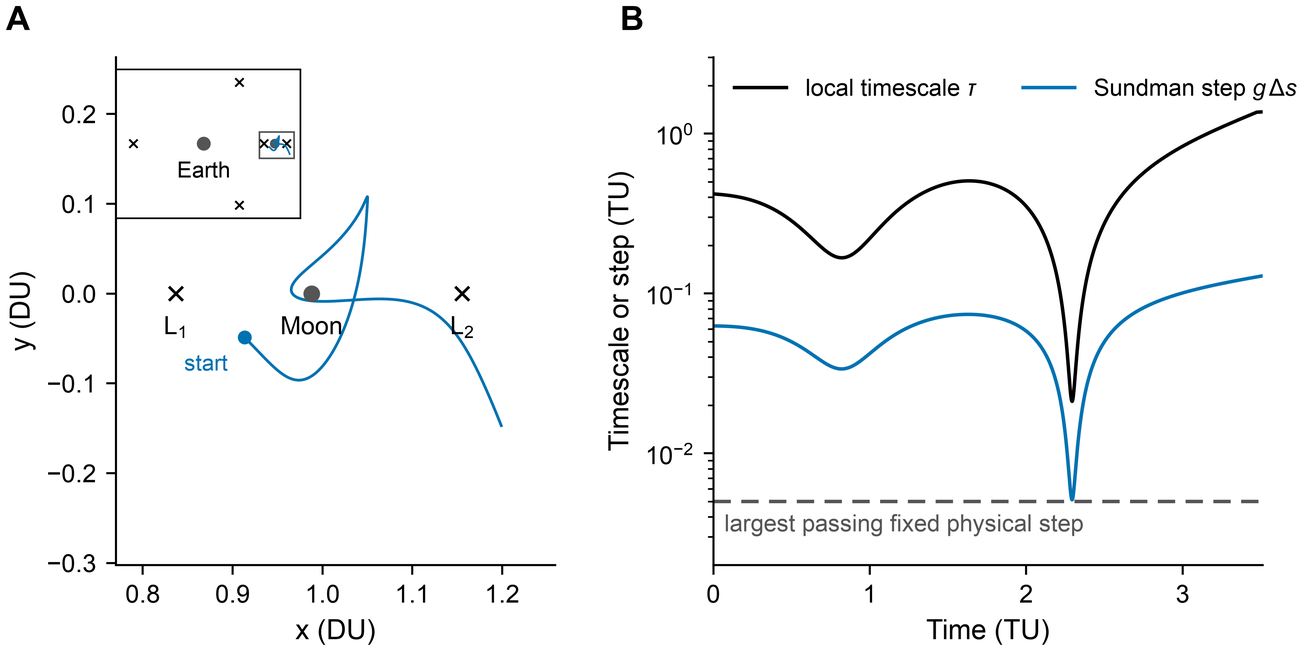
\includegraphics[width=\linewidth]{figures/draft/Fig1.png}\fi
\caption{{\bf A close lunar pass compresses the local timescale by orders of magnitude.}
(A) One trajectory of the Study C confirmation set (horizon 3.51 TU, closest lunar approach 0.018 DU, timescale range $\Delta_{\tau} = 12.5$) in the rotating $x$--$y$ plane near the Moon, with $L_1$ and $L_2$; the inset shows the whole frame with the Earth, the Moon, $L_1$--$L_5$ and the zoomed region. The trajectory was chosen by a fixed rule: among the 141 trajectories of the libration-point branch with one lunar flyby below 0.05 DU, a horizon of 3--8 TU and uncensored labels, the one with the median $\Delta_{\tau}$. (B) Along the same trajectory: the local timescale $\tau(t)$ of Eq~(\ref{eq:tau}) (black), the physical step $g\,\Delta s$ of the Sundman-time integrator at its largest passing fictitious step (blue; Eq~(\ref{eq:sundman})), and the largest fixed physical RK4 step that meets the 100 km tolerance (dashed). Logarithmic axis. DU, distance unit (384,400 km); TU, time unit (4.348 days).}
\label{fig1}
\end{figure}

\subsection*{Trajectory sampling and datasets}
Initial conditions were drawn from a fixed mixture. With probability 0.55 a state was drawn near one of the five libration points chosen uniformly at random, with each position component offset uniformly within $\pm0.1$ DU and each velocity component uniform within $\pm0.15$ DU/TU. With probability 0.20 it was drawn from a wide box ($x \in [-0.5,1.5]$, $y \in [-0.8,0.8]$, $z \in [-0.3,0.3]$ DU, velocity components within $\pm0.5$ DU/TU). With probability 0.25 it was placed near the Moon, at a distance log-uniform between 1.2 lunar radii and 0.15 DU in a uniformly random direction, with velocity components within $\pm0.6$ DU/TU. The horizon $T$ was drawn log-uniformly between 1 and 20 TU (about 4 to 87 days). A trajectory was usable when its reference solution reached $T$; trajectories whose reference collided or escaped before $T$ (about 19\% of each draw, concentrated in Hill regime I) were excluded from the step-size tests and analysed separately in Study C. Because this mixture is synthetic, every share reported below describes this population and not a mission catalogue.

Table~\ref{table1} lists the datasets. Each study fitted and selected on its own development data and ran each confirmatory test once on data generated with new seeds. Study C added an enriched training set that oversampled near-Moon states (mixture weights 0.29, 0.11 and 0.60), reweighted to the natural mixture during fitting. In total about 325,000 Earth--Moon initial conditions were generated for the four studies.

\begin{table}[!ht]
\centering
\caption{{\bf Datasets.}}
\small
\begin{tabular}{|l|L{1.35in}|r|r|r|L{2.15in}|}
\hline
\textbf{Study} & \textbf{Dataset (name in text)} & \textbf{Seed} & \textbf{Candidates} & \textbf{Usable} & \textbf{Role} \\ \thickhline
A & development and locked set & 12 & 20,000 & -- & fitting, calibration (2,000 rows); 5,000 locked rows (4,065 usable) for H1--H2 \\ \hline
A & replication sets & 13, 15 & 20,000 each & -- & secondary replication (S1 Appendix) \\ \hline
B & exploration set & 21 & 20,000 & 16,170 & policy fitting (11,170 rows), all development \\ \hline
B & confirmation set & 22 & 20,000 & 16,161 & tests T1--T5; 2,000 calibration, 14,161 evaluation \\ \hline
B & lock set & 23 & 5,000 & 4,034 & gated policy (descriptive) \\ \hline
C & training set & 41 & 100,000 & 81,111 & fitting \\ \hline
C & enriched training set & 141 & 20,000 & 13,500 & fitting (reweighted) \\ \hline
C & selection set & 42 & 20,000 & 16,190 & model, quantile and guard selection \\ \hline
C & confirmation set & 43 & 20,000 & 16,192 & tests C1--C5; 4,000 calibration, 12,192 evaluation \\ \hline
C & lock set & 44 & 5,000 & 4,020 & one final evaluation \\ \hline
D & selection set & 52 & 10,000 & 8,101 & rule selection, dry runs, written expectations \\ \hline
D & confirmation set & 53 & 20,000 & 16,239 & tests D1, D2 (4,000 calibration, 12,239 evaluation); D4 calibration \\ \hline
D & lock set & 54 & 5,000 & 4,074 & one final evaluation \\ \hline
D & replication set & 55 & 20,000 & 16,253 & test D3 (4,000 calibration, 12,253 evaluation); D4 evaluation \\ \hline
D & JPL periodic orbits & -- & 1,071 members & 942 & test D5 (1,647 runs with $1 \le T \le 20$ TU) \\ \hline
\end{tabular}
\begin{flushleft} Candidates are sampled initial conditions; usable trajectories have a reference solution that reaches the horizon. Study A counted usable rows per analysis; its locked set kept 4,065 of 5,000 rows. Study D fitted no new step-size policy: it used the frozen Study C policies, and its rules were fitted on the Study C training sets. JPL, Jet Propulsion Laboratory; TU, time unit.
\end{flushleft}
\label{table1}
\end{table}

\subsection*{Reference solutions and step-size labels}
The reference for each trajectory was the explicit Runge--Kutta method of order 8 with embedded error estimates of orders 5 and 3 (DOP853)~\cite{hairer1993} in SciPy, run at relative and absolute tolerances of $10^{-13}$ with a maximum step of 0.01 TU and dense output. A run was a violation if its final position differed from the reference by more than $\tol = 100$ km ($2.6015\times10^{-4}$ DU), or if it collided, escaped, produced a non-finite value or reached a cap of 4,000,000 steps. The 100 km tolerance is illustrative, not a mission requirement. It measures integrator error inside the CR3BP, not the accuracy of a real trajectory: against the ephemeris of the CAPSTONE spacecraft retrieved from the Jet Propulsion Laboratory (JPL) Horizons system~\cite{giorgini1996} over 14 days, the CR3BP propagated from observed states drifted by a median of 2,066 km at lags up to 0.25 TU and 50,046 km at 3--5 TU.

The references were checked in three ways. In Study B a Radau IIA solution at $10^{-12}$ agreed with the reference to at most 0.003 km on 600 usable trajectories, and the event type and time agreed on all of 300 colliding or escaping ones. Every trajectory carried a second DOP853 solution (tolerance $10^{-12}$, maximum step 0.005 TU) as a per-trajectory flag. In Study D the 1\% of trajectories with the largest product $\lambda T$ of FTLE and horizon (163 trajectories, $\lambda T \ge 10.8$) were re-integrated with DOP853 at the tightest tolerance SciPy accepts (step at most 0.002 TU) and with LSODA at $10^{-13}$; the largest disagreements were 0.007 km and 0.23 km.

The label of a trajectory for a fixed-step integrator is the largest step that meets the tolerance. Because the final error is not always monotone in the step, we used a locally monotone definition: on a geometric grid with ratio $2^{1/4}$ starting at the ceiling $\min(T, 2\ \mathrm{TU})$ (for the Sundman-time integrator, the fictitious-step range $[10^{-4}, 4]$), the label is the largest grid value that passes together with its eight finer neighbours (two octaves), refined by up to six points towards the next coarser grid value while every finer refinement point still passes. A label is censored when the largest grid value passes. The fraction of trajectories with non-monotone pass/fail sequences on a dense sweep was 1.5\% (3/200) for physical-time RK4 in Study A and 4.0\% (20/500; 95\% interval 2.5--6.1\%) for the Sundman-time integrator in Study D (\nameref{S1_Appendix}).

\subsection*{Integrators}
The fixed-step integrators were the classical fourth-order Runge--Kutta method (RK4; four right-hand side (RHS) evaluations per step) and, in Studies A and B, a second-order leapfrog. The leapfrog splits the rotating-frame Hamiltonian $H = \tfrac{1}{2}|\boldsymbol{p}|^{2} - (x p_{y} - y p_{x}) + V(\boldsymbol{q})$, with canonical momenta $\boldsymbol{p} = (\dot{x}-y,\ \dot{y}+x,\ \dot{z})$ and $V = -(1-\mu)/r_{1} - \mu/r_{2}$, into a kick by $V$ and the exact flow of the remaining terms (free flight followed by a frame rotation). It needs one new RHS evaluation per step when the end-of-step acceleration is reused (Study A charged two), and a finite-difference test of $\Phi^{\mathsf{T}} J \Phi - J$ on 100 states confirmed that it is symplectic to the finite-difference floor ($1.1\times10^{-10}$). Leapfrog was dropped in Study C because, once the safety certificate covered the whole policy, it cost more than it saved in development experiments (\nameref{S1_Appendix}); a plain Sundman transformation is not symplectic, so there is no leapfrog version in Sundman time.

The Sundman-time integrator (Studies C and D) applies RK4 with a constant step $\Delta s$ in a fictitious time $s$ defined by
\begin{equation}
\label{eq:sundman}
\frac{\dd t}{\dd s} = g(\boldsymbol{X}), \qquad
\frac{\dd \boldsymbol{X}}{\dd s} = g(\boldsymbol{X})\,\boldsymbol{F}(\boldsymbol{X}), \qquad
g = \left(\frac{1}{\tau_{1}} + \frac{1}{\tau_{2}} + \frac{1}{\tau_{c}}\right)^{-1},
\end{equation}
where $\boldsymbol{X}$ is the six-dimensional state, $\boldsymbol{F}$ the right-hand side of Eq~(\ref{eq:eom}), $\tau_{1} = \sqrt{r_{1}^{3}/(1-\mu)}$ and $\tau_{2} = \sqrt{r_{2}^{3}/\mu}$ the two-body timescales, and $\tau_{c} = 2$ TU a cap that keeps the physical step finite far from both bodies. The augmented seven-dimensional system $(\boldsymbol{X}, t)$ is integrated by classical RK4 in $s$, so each step costs four RHS evaluations and the physical step $g\,\Delta s$ shrinks in proportion to the local orbital timescale. Close to one body $g \approx \tau_{i} \propto r_{i}^{3/2}$, which corresponds to the generalized Sundman transformation with exponent $\alpha = 3/2$~\cite{berry2002}; the harmonic sum keeps $g$ smooth so that RK4 retains its order. This transformation adapts the step but does not regularize the collision singularity, as the Levi-Civita or Kustaanheimo--Stiefel transformations do~\cite{levicivita1920,kustaanheimo1965}, and it is not symplectic. To end exactly at $T$, before each step the predicted physical step $g(\boldsymbol{X}_{n})\Delta s$ was compared with the remaining time; when $t_{n} + 1.5\,g\,\Delta s \ge T$, or when a fictitious step would overshoot $T$ (the step is discarded and its evaluations still counted), the run finished with $\lceil (T-t_{n})/(g\,\Delta s) \rceil$ equal physical-time RK4 steps. The cap $\tau_{c} = 2$ was chosen on Study C pilot data from $\{0.5, 1, 2\}$; an exploratory sweep in Study D gave nearly the same results for $\tau_{c} \in \{2,4,8\}$ (\nameref{S1_Appendix}).

The adaptive comparators were SciPy's RK45 (the Dormand--Prince 5(4) pair~\cite{dormand1980}) and DOP853 with absolute tolerance $10^{-3}$ times the relative tolerance; their cost is the number of RHS evaluations reported by the solver. A solve needing more than 2,000,000 evaluations was abandoned. Each was run at three tolerances. The oracle-tuned tolerance is, for each trajectory, the loosest relative tolerance (to 0.02 decade) whose final error is within 100 km, found by bracketing and bisection; it uses the answer and therefore bounds the adaptive cost from below. The certified tolerance is one relative tolerance per method certified on the calibration rows by the rule in Eq~(\ref{eq:cert}) over 18 log-spaced values between $10^{-12}$ and $10^{-3}$ (Bonferroni, each value at level $\delta/18$). The equal-risk tolerance is the loosest relative tolerance whose violation rate on the same calibration rows does not exceed the violation rate of the policy it is compared with, refined by four bisection steps in the logarithm; it is recomputed for each policy. The certified and equal-risk tolerances are what a practitioner without the reference could set.

For the wall-clock comparison of Study D, the policy pipeline and the adaptive solvers were compiled with Numba~\cite{lam2015} over identical RHS arithmetic, with the same collision, escape and non-finite checks and no Python calls inside the timed region. The comparators were Dormand--Prince 5(4) with SciPy's step controller (it reproduced SciPy's evaluation counts exactly), Dormand--Prince 5(4) with the proportional--integral (PI) controller of Hairer and Wanner ($\beta = 0.04$)~\cite{hairer1993,gustafsson1988}, which was the primary comparator, and DOP853 with SciPy's tableau and controller.

\subsection*{Features and predictive models}
The state features were the position and velocity, the horizon $T$, the Jacobi constant $C$, $C - C_{L_1}$, $r_{1}$, $r_{2}$ and $r_{1}/r_{2}$. In Study A the FTLE over the horizon, $\lambda = T^{-1}\ln\sqrt{\Lambda_{\max}(\Phi^{\mathsf{T}}\Phi)}$ with $\Phi$ the state-transition matrix from the variational equations, was also a feature; computing it requires integrating the variational equations over the whole horizon, so it is not available before the run~\cite{shadden2005,gawlik2009}. From Study B on it was used only to explain results.

Study C added 13 periapsis features computed analytically from the osculating two-body orbit about each primary. For body $i$ with gravitational parameter $\mathrm{GM}_{1} = 1-\mu$ or $\mathrm{GM}_{2} = \mu$, let $\boldsymbol{r}$ be the position relative to the body and $\boldsymbol{v} = \dot{\boldsymbol{r}}_{\mathrm{rot}} + \hat{\boldsymbol{z}}\times\boldsymbol{r}$ the inertial velocity. With $\boldsymbol{h} = \boldsymbol{r}\times\boldsymbol{v}$, eccentricity vector $\boldsymbol{e} = \boldsymbol{v}\times\boldsymbol{h}/\mathrm{GM} - \boldsymbol{r}/|\boldsymbol{r}|$ and $e = |\boldsymbol{e}|$, the periapsis radius and, for an elliptic orbit with semi-major axis $a$ and mean motion $n = \sqrt{\mathrm{GM}/a^{3}}$, the time to the next periapsis are
\begin{equation}
\label{eq:peri}
r_{p} = \frac{|\boldsymbol{h}|^{2}}{\mathrm{GM}(1+e)}, \qquad
t_{p} =
\begin{cases}
-M/n, & M < 0,\\
(2\pi - M)/n, & M \ge 0,
\end{cases}
\qquad
M = E - e\sin E,
\end{equation}
where the eccentric anomaly $E \in (-\pi,\pi]$ follows from $e\cos E = 1 - |\boldsymbol{r}|/a$ and $e\sin E = \boldsymbol{r}\cdot\boldsymbol{v}/\sqrt{\mathrm{GM}\,a}$. For a hyperbolic orbit the hyperbolic anomaly was used, and an outgoing hyperbola has no future periapsis; near-circular and near-parabolic cases were handled separately (\nameref{S1_Appendix}). For each body the features were $\log_{10} r_{p}$, $\log_{10}\sqrt{r_{p}^{3}/\mathrm{GM}}$, $\min(t_{p}/T, 2)$, an indicator of $t_{p} \le T$, the logarithm of the current distance (relative to the Hill radius $(\mu/3)^{1/3}$ for the Moon) and $e$; the thirteenth feature was the logarithm of the shortest of these periapsis timescales over the two bodies, using the current distance for a body whose periapsis is not reached before $T$. These features cost a few arithmetic operations and no RHS evaluation, and are exact only for two-body motion.

The step predictors were gradient-boosted regression trees~\cite{friedman2001} with histogram binning and the quantile (pinball) loss~\cite{koenker1978} on the logarithm of the label, so that the prediction aims below the median by design. Study A used per-integrator hurdle models (a random-forest classifier with 150 trees deciding whether any step passes, and a regressor at quantile 0.1); Study B used the same class without FTLE. The final Study C policy predicts the logarithm of the fictitious step $\Delta s$ with 25 trees of depth 3, learning rate 0.2 and quantile 0.2 from the 12 state and 13 periapsis features; model class, size and quantile were chosen on the Study C selection set by the median total cost of trajectories that met the tolerance, with candidates whose violation rate exceeded 6\% excluded. A physical-time counterpart (10 trees, RK4 only, with abstention to the certified RK45 when the osculating lunar orbit returns within the horizon with a short periapsis timescale) and a single global fictitious step with no model served as controls.

The physics rules of Study D have the form $\log_{10}\Delta s = b + \boldsymbol{w}\cdot\boldsymbol{f}$, with $\boldsymbol{f}$ a subset of $\log_{10} T$, the Hill regime coded 1--5, the logarithm of the shortest periapsis timescale, the logarithm of the smallest osculating periapsis radius over the two bodies, and $C - C_{L_1}$. Six rules with two to five coefficients were fitted by weighted linear quantile regression (the interior point solver IPX~\cite{schork2020} in HiGHS~\cite{huangfu2018}) on the Study C training sets, with quantile chosen from $\{0.1, 0.2, 0.3, 0.5\}$ on the Study D selection set. The rule chosen as the test arm used $\log_{10}T$, the Hill regime and the logarithm of the periapsis radius (four coefficients, quantile 0.1). A linear quantile model on 33 engineered features (the logarithms of $r_{1}$, $r_{2}$ and $T$, $C - C_{L_1}$, the 13 periapsis features, and the products of these with $\log_{10} T$) was frozen as a descriptive arm.

The cost of features and inference was measured as wall time per call divided by the wall time of one compiled RHS evaluation in the same session (median of repeated measurements on an idle machine) and charged once per trajectory in RHS-equivalents. It was pinned in advance in each study: 1,128 RHS-equivalents for the scikit-learn model of Study B, 15.04 for the compiled 25-tree Study C policy (of which 3.6 for computing the features), and 11.74 for the physical-time policy. Study D re-measured all arms in one session on a machine whose RHS evaluation was faster (18.3 against 25--28 ns), so the same 25-tree model cost 16.09 RHS-equivalents there; the rules cost 2.05--7.43 and the linear arm 11.39.

\subsection*{Failure-rate certification}
The predicted step was multiplied by a safety scale $s \le 1$ chosen so that the probability of a violation is controlled. Let $s_{1} < s_{2} < \dots < s_{m}$ be a grid (in Studies C and D, $s_{k} = 0.1\cdot2^{(k-1)/8}$ for $k = 1,\dots,27$, and $s_{28} = 1$), let $n$ be the number of calibration trajectories and $V(s)$ the number of them that violate when run end to end at scale $s$. For each $s_{k}$ in ascending order the null hypothesis that the violation rate exceeds $\alpha$ was tested with the exact one-sided binomial p-value
\begin{equation}
\label{eq:cert}
p(s_{k}) = \Pr\left[\mathrm{Bin}(n,\alpha) \le V(s_{k})\right],
\qquad
\hat{s} = \max\left\{ s_{k} : p(s_{j}) \le \delta \ \text{for all}\ j \le k \right\},
\end{equation}
with $\alpha = 0.05$ and $\delta = 0.1$ (the symbol $\delta$ is used only for this level). This is fixed-sequence testing within the Learn-then-Test framework~\cite{angelopoulos2025}: if calibration and test trajectories are exchangeable, the violation rate at $\hat{s}$ exceeds $\alpha$ with probability at most $\delta$. The guarantee is marginal over the sampling distribution; it says nothing about the rate in a subpopulation. Studies A and B used the Bonferroni version (each value of an 18-value grid between 0.02 and 1 tested alone at level $\delta/18$, and the largest certified value kept), which needs no ordering of the risks but has less power; the global fixed-step controls were certified on their own grids by the rule of their study. A violation in calibration included any run that collided, escaped, was non-finite, hit the step cap, or was handed to a fallback solver that then violated.

The conditional certificate of Study D (D4) partitioned trajectories into strata using only quantities known before integration: regime group (I, II--III, IV--V), lunar class from the osculating orbit (predicted collision, periapsis below 0.05 DU reached before $T$, periapsis 0.05--0.17 DU, or far) and horizon band (1--3, 3--8, 8--20 TU). Base cells with fewer than 400 calibration trajectories were merged by a fixed rule, which gave $G = 17$ strata, each with at least 411 calibration trajectories. Each stratum certified its own scale by Eq~(\ref{eq:cert}) at level $\delta/G$; a stratum without a certified scale or with fewer than 150 calibration trajectories would have been handed to RK45 at the certified tolerance (none was). Scales were certified on all usable trajectories of the Study D confirmation set and evaluated on all usable trajectories of the replication set.

\subsection*{Cost accounting and decomposition of the cost gap}
Cost was the number of RHS evaluations, with the policy's feature and model cost added in RHS-equivalents. A trajectory counted as cheaper for the policy only if the policy run also met the tolerance. The preregistered cost statistic was the share of trajectories on which the policy was cheaper, because it states how often a user drawing a trajectory from the population gains by using the policy and is not driven by the few very expensive trajectories; for the same reason it does not measure the cost of a batch, which those trajectories dominate. We therefore also report, as post hoc summaries of the sealed ledgers, the ratio of totals (comparator evaluations summed over the evaluation trajectories divided by the policy's, overhead and violating runs included; above 1 favours the policy) and the mean of $\log_{10}$ of the per-trajectory ratio, with 95\% bootstrap intervals over trajectories (\nameref{S4_Table}). Ratios are reported in dex, a base-10 logarithmic unit: a difference of 0.1 dex is a factor of $10^{0.1} \approx 1.26$.

For the physical-time policy of Study B the logarithm of the cost ratio against an adaptive solve of cost $C_{\mathrm{ad}}$ decomposes exactly as
\begin{equation}
\label{eq:decomp}
\log_{10}\frac{C_{\mathrm{tot}}}{C_{\mathrm{ad}}} =
\underbrace{\log_{10}\frac{C^{*}_{\mathrm{fix}}}{C_{\mathrm{ad}}}}_{P}
+ \underbrace{\log_{10}\frac{e_{k}/d^{*}_{k}}{e_{k^{*}}/d^{*}_{k^{*}}}}_{S}
+ \underbrace{\log_{10}\frac{d^{*}_{k}}{\hat{d}_{k}}}_{Q}
+ \underbrace{\log_{10}\frac{1}{s_{k}}}_{K}
+ \underbrace{\log_{10}\left(1 + \frac{C_{\mathrm{feat}} + C_{\mathrm{pred}}}{C_{\mathrm{int}}}\right)}_{O}
+ R,
\end{equation}
where $d^{*}_{k}$ is the label and $e_{k}$ the evaluations per step of integrator $k$, $k$ is the integrator the policy chose and $k^{*}$ the cheaper one at its label, $C^{*}_{\mathrm{fix}} = \min_{k} e_{k}\lceil T/d^{*}_{k}\rceil$ is the cost of the best single fixed step chosen with perfect knowledge (Studies A and B offered RK4 and leapfrog, with $e_{\mathrm{RK4}} = 4$, and $e_{\mathrm{leapfrog}} = 2$ in Study A and 1 in Study B, where the end-of-step acceleration was reused), $\hat{d}_{k}$ is the predicted step, $s_{k}$ the certified scale, $C_{\mathrm{int}}$ the integration cost and $C_{\mathrm{feat}} + C_{\mathrm{pred}}$ the overhead. The terms are the paradigm gap $P$ (the best any single physical step can do), selection $S$, prediction $Q$, safety scale $K$ and overhead $O$; $R$ collects rounding of the step count. For the Sundman-time policy there is no selection term, $P$ is replaced by $P_{s} = \log_{10}(C^{*}_{s}/C_{\mathrm{ad}})$ with $C^{*}_{s}$ the counted cost of the run at the oracle fictitious step, and $R$ also absorbs the landing steps. Means of the terms add to the mean total; medians do not.

\subsection*{Wall-clock timing protocol}
Study D timed every evaluation trajectory of the confirmation set on a single thread of an Apple M5 (10 cores, macOS) with Numba 0.67. The time of a trajectory was the minimum over three repeats of an inner loop of about 0.5 ms; the policy time covered features, tree inference, scaling and integration. The adaptive tolerances were recalibrated for the compiled solvers on the same 4,000 calibration trajectories. The throughput ratio is the total comparator time divided by the total policy time over the same trajectories; values above 1 favour the policy. The step was guarded to start only when the 1-minute load average was below 1.5; it was launched with the guard relaxed to 1.6 because the load hovered at 1.50 with the processor 94.5\% idle, and the recorded load at the start was 1.499 (a dated deviation in the preregistration). Batches of $10^{3}$, $10^{4}$ and $10^{5}$ trajectories were timed on one and ten threads (7 repeats). No GPU or vector kernel was written; the lane efficiency of a lock-step batch was modelled from measured step counts.

\subsection*{Periodic orbits and chaos maps}
Test D5 used the JPL Three-Body Periodic Orbits API~\cite{jplperiodic} for the Earth--Moon system: 21 streams grouped into 11 families (halo $L_1$ and $L_2$, Lyapunov $L_1$ and $L_2$, vertical $L_1$ and $L_2$, axial $L_1$ and $L_2$, distant retrograde, butterfly, and resonant orbits). From each stream 50 members evenly spaced along the family were taken, disjoint from a dry-run sample used to write the expectations. The states were integrated at JPL's mass ratio ($1.215058561\times10^{-2}$, relative difference $2.1\times10^{-8}$ from ours); a member was dropped before any policy run if one period at $10^{-13}$ did not close to $10^{-8}$ in the maximum norm, if it reached a collision radius, or if the reference stopped (129 of 1,071 members). Horizons of 1, 2, 5, 10 and 20 periods were used when they lay between 1 and 20 TU, the training range. A run was excluded when a second DOP853 reference (tolerance $10^{-12}$, step at most 0.004 TU) disagreed with the first by more than 5 km (102 of 1,749 runs). The frozen Study C policy, scale and comparator tolerances were applied unchanged. The statistic was the family-balanced violation rate (mean over families of the family rate), with all horizons of a member and the mirror images of a halo or butterfly member treated as one cluster.

The chaos maps of Study D (exploratory) used the surface of section $y = 0$, $z = \dot{z} = 0$, $\dot{y} > 0$ at $C = 3.19$, 3.10 and 2.95, on a $110\times110$ grid in $(x,\dot{x})$ with $\dot{y}$ fixed by $C$, a horizon of 8 TU, and the FTLE from the variational equations.

\subsection*{Preregistration and statistical analysis}
Each study was preregistered in a document that stated the hypotheses, tests, data, policies and decision rules, together with the outcome expected from a dry run on development data. Before the confirmatory run a script recorded the SHA-256 hashes of the document, every source file, the frozen models and the datasets (sealed 2026 Oct 23, 25, 27 and 28 for Studies A--D); the confirmatory runner refused to start if any hash had changed and logged each step, which ran once. Changes after a seal are dated deviations in each document; none altered a confirmatory computation (\nameref{S1_Appendix}). These were internal preregistrations deposited with the code, not registered reports. Analyses not in a preregistered test family are labelled exploratory.

Each of Studies B, C and D had a family of five one-sided confirmatory tests, with the direction fixed in the preregistration, and controlled the familywise error rate at $\alpha = 0.05$ with the Holm procedure~\cite{holm1979}. Study A judged its cost hypotheses by preregistered decision thresholds (at least 90\% of trajectories within tolerance and at least 50\% cheaper than each comparator). Shares were tested with exact binomial tests and reported with Clopper--Pearson 95\% confidence intervals (CIs)~\cite{clopper1934}. Paired cost differences and differences of medians were tested with one-sided bootstrap tests over trajectories~\cite{efron1979} (4,000 resamples; the p-value is the share of resamples with a difference in the null direction, with a floor of $2.5\times10^{-4}$), and 95\% intervals are percentile bootstrap intervals. Study B used permutation tests (10,000 permutations) for Spearman rank correlations~\cite{spearman1904}, Mann--Whitney tests~\cite{mann1947} and a two-proportion z-test for the location contrasts, and a chi-square homogeneity test; intersection--union tests take the largest component p-value. The unit of analysis is the trajectory; in D5 it is the periodic-orbit member, resampled within family. Reference-divergent trajectories were excluded from all cost tests and analysed separately; untrusted periodic-orbit references were excluded and listed. p-values below 0.001 are reported as $p < 0.001$; bootstrap and permutation p-values at their floor are bounds.

The analysis used Python 3.11.16 with NumPy 2.4.6~\cite{harris2020}, SciPy 1.17.1~\cite{virtanen2020}, scikit-learn 1.9.0~\cite{pedregosa2011}, pandas 3.0.5~\cite{mckinney2010}, Numba 0.67.0 (llvmlite 0.49.0)~\cite{lam2015} and Matplotlib 3.11.1~\cite{hunter2007}; Study A ran under Python 3.13.13 with NumPy 2.5.1, pandas 3.0.5 and scikit-learn 1.9.0, as recorded in its run manifests; Studies B--D used the versions above. The IAS15 baseline used REBOUND 5.2.2~\cite{rein2012,rein2015}. The code, the sealed preregistrations, the seal manifests, the frozen models and the processed data behind every figure and statistic are deposited at [repository DOI to be assigned].

\subsection*{Use of AI tools}
The analysis code of all four studies (data generation, integrators, models, certification, statistical tests and figure scripts) was written with the assistance of a large language model coding agent (Claude Sonnet 5.5, Anthropic) working under the author's direction, and the text of this manuscript was drafted with the assistance of Claude Opus 5.5 (Anthropic) from the project's sealed reports and result files. The author designed the studies, set the hypotheses, and reviewed the code, results and text. Validity was checked by unit tests of every kernel (including step-for-step agreement of the compiled solvers with SciPy, fourth-order convergence of the Sundman-time integrator, and the exactness of the cost decomposition), by the preregistration seals, which prevented any change to sealed code between the dry run and the confirmatory run, and by recomputing every number in this article from the result files.

\section*{Results}
Table~\ref{table2} lists every preregistered confirmatory test with its outcome.

\begin{table}[!ht]
\centering
\caption{{\bf Preregistered confirmatory tests.}}
\small
\begin{tabular}{|L{0.55in}|L{1.95in}|L{1.9in}|L{0.5in}|L{0.75in}|}
\hline
\textbf{Test} & \textbf{Hypothesis (one-sided)} & \textbf{Result (95\% CI)} & \textbf{p (Holm)} & \textbf{Verdict} \\ \thickhline
A-H1 & ML step with FTLE cost charged: $\ge$90\% within tolerance and cheaper than each adaptive solver on $\ge$50\% & within 959/996 (96.3\%); cheaper 0/996 against each of 4 & decision rule & not supported \\ \hline
A-H1$'$a & same without FTLE, inference cost charged (added post hoc) & within 960/999 (96.1\%); cheaper 0/999 against each of 4 & decision rule & not supported \\ \hline
A-H2 & certified scales give $\le$5\% violations & RK4 17/500 (3.4\%, 2.0--5.4); leapfrog 19/498 (3.8\%, 2.3--5.9) & reported & point estimates met \\ \hline
A-H3 & removing FTLE lowers RK4 $R^{2}$ (whole CI below 0) & $\Delta R^{2} = -0.25$ ($-0.54$ to 0.04) & reported & not met \\ \thickhline
B-T1 & oracle fixed step cheaper than oracle-tuned RK45 on $<$50\%, and gap rises with $\Delta_{\tau}$ & 3,658/14,160 (25.8\%, 25.1--26.6); $\rho = 0.909$ & $<$0.001 & supported \\ \hline
B-T2 & label spread under 3.8 km perturbations rises with $\lambda T$ & $\rho = 0.41$ ($n = 443$) & $<$0.001 & supported (sign only) \\ \hline
B-T3 & per-regime scales cut cost at equal certified risk & +0.073 dex costlier (0.072--0.075) & 1.000 & not supported \\ \hline
B-T4 & gap and violations larger near the Moon and in regimes II--III & violations 394/2,552 (15.4\%) vs 152/11,609 (1.3\%) & $<$0.001 & supported \\ \hline
B-T5 & paradigm and integration gaps rise with horizon & mean $\rho$ 0.908 and 0.727 & $<$0.001 & supported \\ \thickhline
C-C1 & periapsis features lower median step error & 0.037 dex (0.027--0.048) & $<$0.001 & supported \\ \hline
C-C2 & physical-time policy cheaper than equal-risk RK45 on $>$50\% & 3,855/12,192 (31.6\%, 30.8--32.5) & 1.000 & not supported \\ \hline
C-C3 & oracle Sundman step cheaper than oracle-tuned RK45 on $>$50\%, and gap no longer tracks $\Delta_{\tau}$ & 6,234/12,190 (51.1\%, 50.2--52.0); $\rho$ 0.225 vs 0.911 & 0.012 & supported \\ \hline
C-C4 & Sundman policy cheaper than equal-risk RK45 on $>$50\% & 8,707/12,192 (71.4\%, 70.6--72.2) & $<$0.001 & supported \\ \hline
C-C5 & model cheaper than one global certified step & 0.306 dex (0.302--0.310) & $<$0.001 & supported \\ \thickhline
D-D1 & model cheaper than the best physics rule & 0.072 dex (0.069--0.074) & $<$0.001 & supported \\ \hline
D-D2 & compiled throughput above compiled DP5(4)-PI at equal risk & ratio 0.885 (0.862--0.908) & 1.000 & not supported \\ \hline
D-D3 & C4 replicates on new data & 8,768/12,253 (71.6\%, 70.8--72.4) & $<$0.001 & supported \\ \hline
D-D4 & every free stratum $<$7\% violations and cheaper than equal-risk RK45 on $>$50\% & worst stratum 98/3,142 (3.1\%); 10,792/16,253 (66.4\%, 65.7--67.1) & $<$0.001 & supported \\ \hline
D-D5 & family-balanced violation rate on JPL periodic orbits $<$10\% & 70.0\% (67.8--72.3), 1,647 runs & 1.000 & not supported \\ \hline
\end{tabular}
\begin{flushleft} Study A used decision thresholds, not p-values; H1$'$a was added after development data had been seen (dated deviation). Holm adjustment is within each study's family of five tests. $\Delta_{\tau}$, timescale range (Eq~(\ref{eq:tau})); $\lambda T$, FTLE times horizon; $\rho$, Spearman correlation; DP5(4)-PI, compiled Dormand--Prince 5(4) with a proportional--integral step controller; FTLE, finite-time Lyapunov exponent; JPL, Jet Propulsion Laboratory; ML, machine learning.
\end{flushleft}
\label{table2}
\end{table}

\subsection*{A fixed physical step never cost less than adaptive integration}
Study A tested the original design: a hurdle model with FTLE among its features chose between RK4 and leapfrog and predicted a step, which was multiplied by a certified scale. On the locked set the scaled policy met the tolerance on 959/996 trajectories of the cost sample (96.3\%; 95\% CI 94.9--97.4\%), but it was cheaper than RK45 and DOP853, at the oracle-tuned and at the certified tolerance, on 0/996 trajectories in each comparison (Table~\ref{table2}). The FTLE alone made this inevitable: on 80 development trajectories it cost more than a whole DOP853 solve on every one, by a median factor of about 70. A post hoc variant without FTLE, charging the measured inference cost (about 591 RHS-equivalents per trajectory against median oracle-tuned adaptive costs of 146 for RK45 and 122 for DOP853), was also cheaper on 0/999 trajectories. Removing FTLE did not change predictive quality by an amount the preregistered test could detect: the change in $R^{2}$ of the RK4 step was $-0.25$ (95\% CI $-0.54$ to 0.04), and the change in integrator-selection accuracy was 0.008 ($-0.009$ to 0.024). The certified scales kept the violation rate at 17/500 (3.4\%) for RK4 and 19/498 (3.8\%) for leapfrog, although the upper confidence bounds (5.4\% and 5.9\%) did not exclude rates above 5\%.

\subsection*{The cost gap and the timescale range}
Study B asked why. With features restricted to the initial state and every cost charged, the policy was cheaper than an adaptive solver on 0/14,161 trajectories of the confirmation set against all six comparator settings. The mean decomposition of Eq~(\ref{eq:decomp}) against the oracle-tuned RK45, over the 13,540 trajectories that met the tolerance and had every term, was $+1.41$ dex (95\% CI 1.40--1.41), a factor of about 26: paradigm $+0.21$ (0.21--0.22), selection $+0.03$, prediction $+0.38$ (0.37--0.38), safety scale $+0.30$, overhead $+0.50$ (0.49--0.51) and rounding $-0.01$.

The paradigm term behaved as the timescale-range hypothesis predicts (test T1). A single fixed step chosen with perfect knowledge was cheaper than the oracle-tuned RK45 on only 3,658/14,160 trajectories (25.8\%; 25.1--26.6\%) and than the oracle-tuned DOP853 on 3,740/14,160 (26.4\%; 25.7--27.1\%), and its cost penalty rose with the timescale range: Spearman $\rho = 0.909$ between $\log_{10}\Delta_{\tau}$ and the paradigm gap, with an ordinary least-squares slope of 0.904 (95\% CI 0.898--0.910) dex per dex (Fig~\ref{fig2}A). The same initial states relabelled at horizons of 1, 2, 5, 10 and 20 TU showed the gap rising with the horizon (T5; mean per-state $\rho = 0.908$, 95\% CI 0.900--0.914, over 2,326 states), from $-0.20$ dex at 1 TU to $+0.34$ dex at 20 TU in the median.

\begin{figure}[!h]
\ifdraftfigs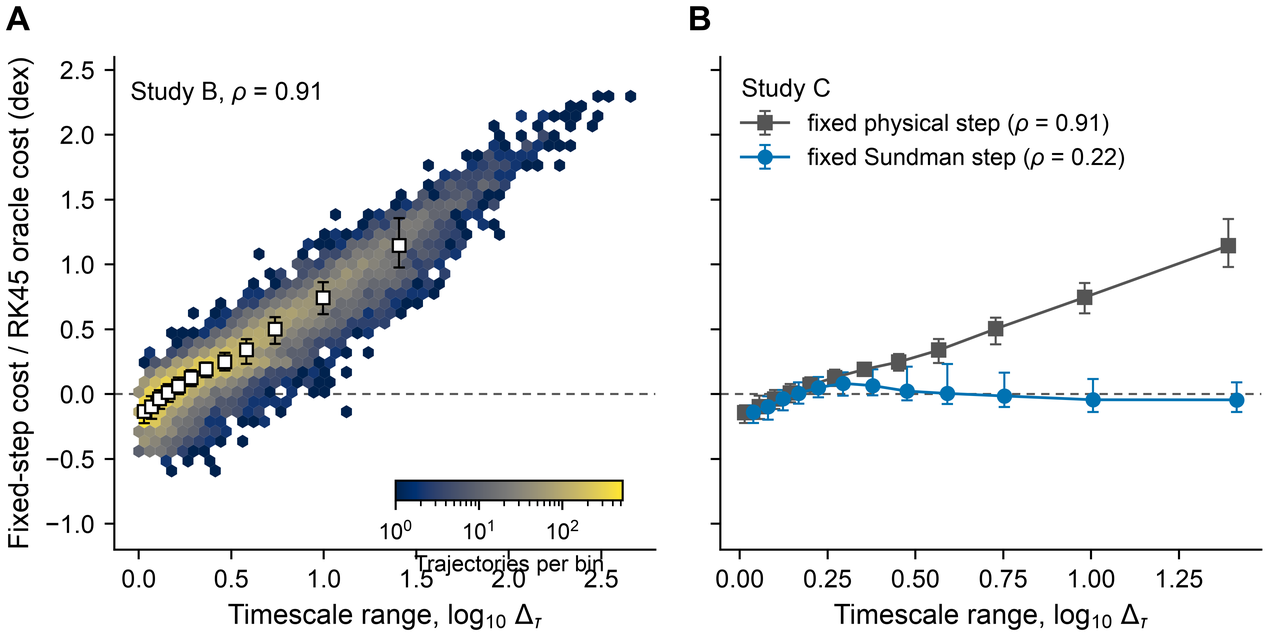
\includegraphics[width=\linewidth]{figures/draft/Fig2.png}\fi
\caption{{\bf The penalty of one fixed physical step tracks the timescale range; in Sundman time it does not.}
The gap is $\log_{10}$ of the cost at the oracle fixed step divided by the cost of RK45 at the per-trajectory oracle-tuned tolerance (dex); values above 0 (dashed line) mean the fixed step costs more. (A) Study B confirmation set ($n = 14,160$), oracle fixed physical step against $\log_{10}\Delta_{\tau}$ (Eq~(\ref{eq:tau})): hexagonal-bin counts (colour, logarithmic scale) with medians (white squares) and interquartile ranges (bars) in 12 equal-count bins; Spearman $\rho = 0.91$. (B) Study C confirmation set ($n = 12,190$): medians and interquartile ranges in the same bins for the oracle fixed physical step (grey squares, $\rho = 0.91$) and the oracle fixed Sundman step (blue circles, $\rho = 0.22$).}
\label{fig2}
\end{figure}

How much the paradigm term matters depends on how the adaptive solver is tuned. Against one certified tolerance for all trajectories, rather than an oracle tolerance per trajectory, the same perfect fixed step was cheaper than RK45 on 9,609/14,160 trajectories (67.9\%) and than DOP853 on 7,902/14,160 (55.8\%). The claim that a single step cannot win therefore holds against an oracle-tuned adaptive solver but not against a realistically tuned one; against the latter the losses came from prediction, the safety scale and overhead, the three largest terms of the decomposition (Fig~\ref{fig3}A).

\begin{figure}[!h]
\ifdraftfigs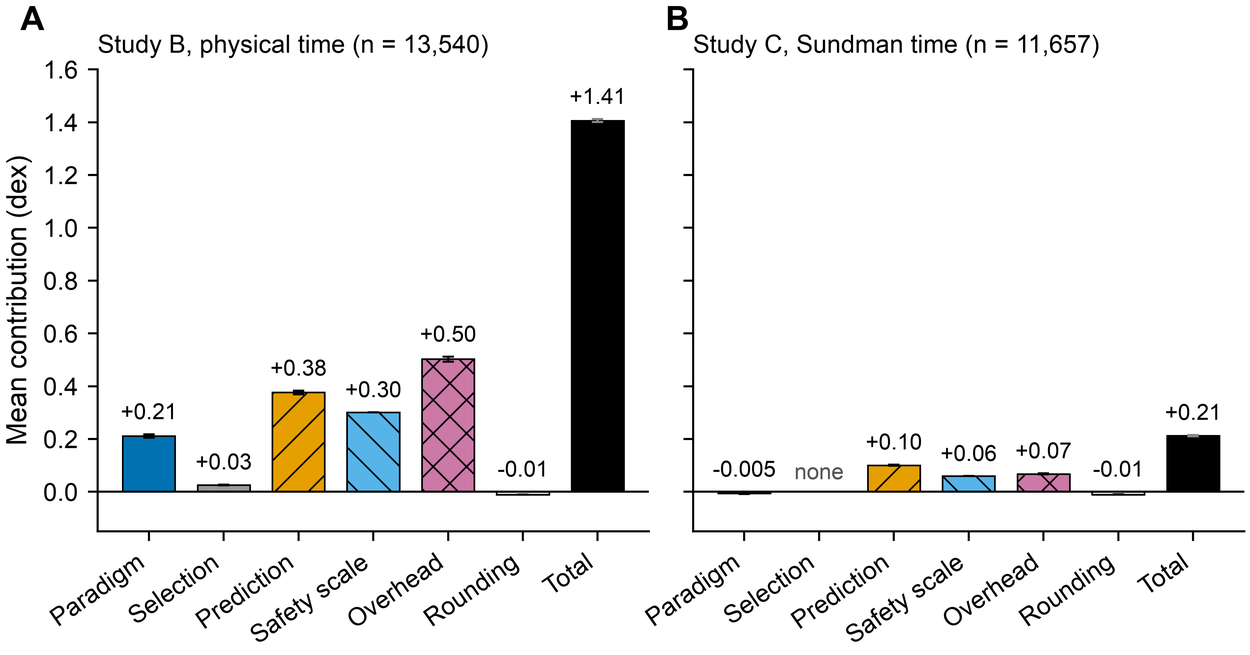
\includegraphics[width=\linewidth]{figures/draft/Fig3.png}\fi
\caption{{\bf Where the cost of a predicted fixed step goes, before and after the time transformation.}
Mean of each term of Eq~(\ref{eq:decomp}) in dex against RK45 at the oracle-tuned tolerance, over trajectories that met the tolerance and had every term; positive values are costs relative to the adaptive solver, and the number above each bar is the mean. Error bars are 95\% percentile bootstrap intervals over trajectories (4,000 resamples); the safety-scale term has no spread because one scale applies to all trajectories. (A) Study B physical-time policy ($n = 13,540$; total $+1.41$ dex). (B) Study C Sundman-time policy ($n = 11,657$; total $+0.21$ dex), which has no selection term.}
\label{fig3}
\end{figure}

Where the gap and the failures concentrate was tested in T4 (Fig~\ref{fig4}). The median paradigm gap was $+0.48$ dex for trajectories whose closest lunar approach was below 0.17 DU and $+0.07$ dex beyond, and $+0.24$ against $+0.06$ dex in Hill regimes II--III against IV--V. Violations occurred on 394/2,552 trajectories (15.4\%) that passed within 0.05 DU of the Moon and on 152/11,609 (1.3\%) of the rest. They were step-overs: the ratio of the scaled step to the minimum timescale separated violations from non-violations with an area under the receiver operating characteristic curve (AUC) of 0.85. The safety scale could not be targeted from the initial state either (T3): scales certified per Hill regime cost 0.073 dex more (95\% CI 0.072--0.075) than one global scale over 13,605 paired trajectories, a cost we attribute to splitting the error budget $\delta$ over the groups. The label itself was stable: 16 perturbed copies of 443 trajectories at 3.8 km and 1 cm/s gave a standard deviation of the label of at most 0.14 dex, while the model's median error was 0.32 dex, so the prediction error came from the features, not from an information floor in the initial state (T2 is supported in sign only). In exploratory work on the Study B exploration set, adding features that require the trajectory (closest approach, timescales, transit counts) cut the median error from 0.294 to 0.057 dex.

\begin{figure}[!h]
\ifdraftfigs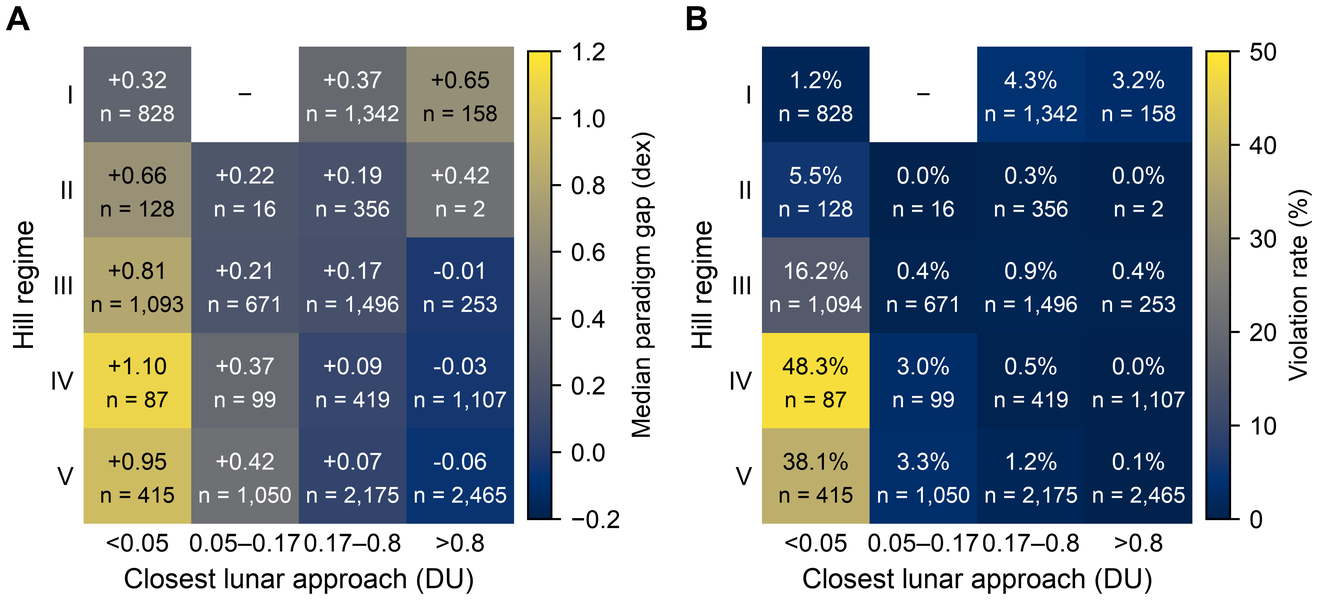
\includegraphics[width=\linewidth]{figures/draft/Fig4.png}\fi
\caption{{\bf The fixed-step penalty and the failures concentrate at close lunar passes.}
Study B confirmation set, cells of Hill regime (rows I--V, from the Jacobi constant) by closest lunar approach along the reference trajectory (columns, DU). (A) Median paradigm gap, $\log_{10}$ of the oracle fixed-step cost over the cost of RK45 at the oracle-tuned tolerance ($n = 14,160$). (B) Violation rate of the certified physical-time policy ($n = 14,161$). Each cell prints its value and its number of trajectories; a dash marks an empty cell. The empty cell is physical (post hoc check): for $C > C_{L_1}$ the zero-velocity surface separates a lunar region, in which every usable regime-I trajectory came within 0.047 DU of the Moon, from the Earth region, whose trajectories stayed beyond 0.169 DU (2,675 usable regime-I trajectories; the one at 0.1691 DU is a calibration trajectory). DU, distance unit.}
\label{fig4}
\end{figure}

\subsection*{Sundman time removes the timescale penalty}
Study C attacked the two largest terms of Eq~(\ref{eq:decomp}). The paradigm term was addressed by integrating in Sundman time, where one constant fictitious step yields physical steps that follow the local timescale (Eq~(\ref{eq:sundman})), and the prediction term by the analytic periapsis features, which tell the model whether and how closely the trajectory will approach a body before $T$. The overhead term was reduced by a compiled 25-tree model.

The time transformation removed the dependence on the timescale range (C3). The rank correlation between $\log_{10}\Delta_{\tau}$ and the gap of the oracle fixed step fell from 0.911 in physical time to 0.225 in Sundman time on the same trajectories (difference 0.686, 95\% CI 0.667--0.705; Fig~\ref{fig2}B), and the mean paradigm term against the oracle-tuned RK45 fell from $+0.12$ dex for the physical step on the same trajectories ($+0.21$ in Study B) to $-0.005$ dex. The oracle Sundman step was cheaper than the oracle-tuned RK45 on 6,234/12,190 trajectories (51.1\%; 50.2--52.0\%), a narrow pass of the 50\% threshold that the pilot data had flagged as a coin flip (Holm-adjusted $p = 0.012$ for the conjunction). The target also became easier to predict: the standard deviation of the logarithm of the label was 0.33 dex for the fictitious step against 0.91 dex for the physical RK4 step. The periapsis features lowered the median absolute error of the predicted physical RK4 step from 0.319 to 0.282 dex (C1; difference 0.037 dex, 95\% CI 0.027--0.048, $n = 12,191$), a small gain because the model that fitted within the overhead budget was small.

The Sundman-time policy (certified scale 0.872, overhead 15.04 RHS-equivalents) was cheaper than RK45 at the equal-risk tolerance on 8,707/12,192 trajectories of the confirmation set (71.4\%; 70.6--72.2\%; C4, $p < 0.001$) at a realized violation rate of 535/12,192 (4.39\%; 4.03--4.77\%) (Fig~\ref{fig5}A). It was cheaper than RK45 at the certified tolerance on 10,045/12,192 (82.4\%), than DOP853 at the equal-risk tolerance on 6,166/12,192 (50.6\%), and than DOP853 at the certified tolerance on 7,147/12,192 (58.6\%). It was not cheaper than the oracle-tuned solvers, which choose their tolerance knowing the answer: 1,058/12,192 (8.7\%) against RK45 and 747/12,192 (6.1\%) against DOP853. The mean gap against the oracle-tuned RK45 fell from $+1.41$ to $+0.21$ dex (paradigm $-0.005$, prediction $+0.10$, safety scale $+0.06$, overhead $+0.07$, rounding $-0.01$; Fig~\ref{fig3}B). The same ideas in physical time were not enough: the physical-time policy was cheaper than equal-risk RK45 on 3,855/12,192 trajectories (31.6\%; C2, not supported). The model added value over a single certified global fictitious step, saving 0.306 dex (0.302--0.310) and being cheaper on 10,213/11,359 paired trajectories (89.9\%; C5).

\begin{figure}[!h]
\ifdraftfigs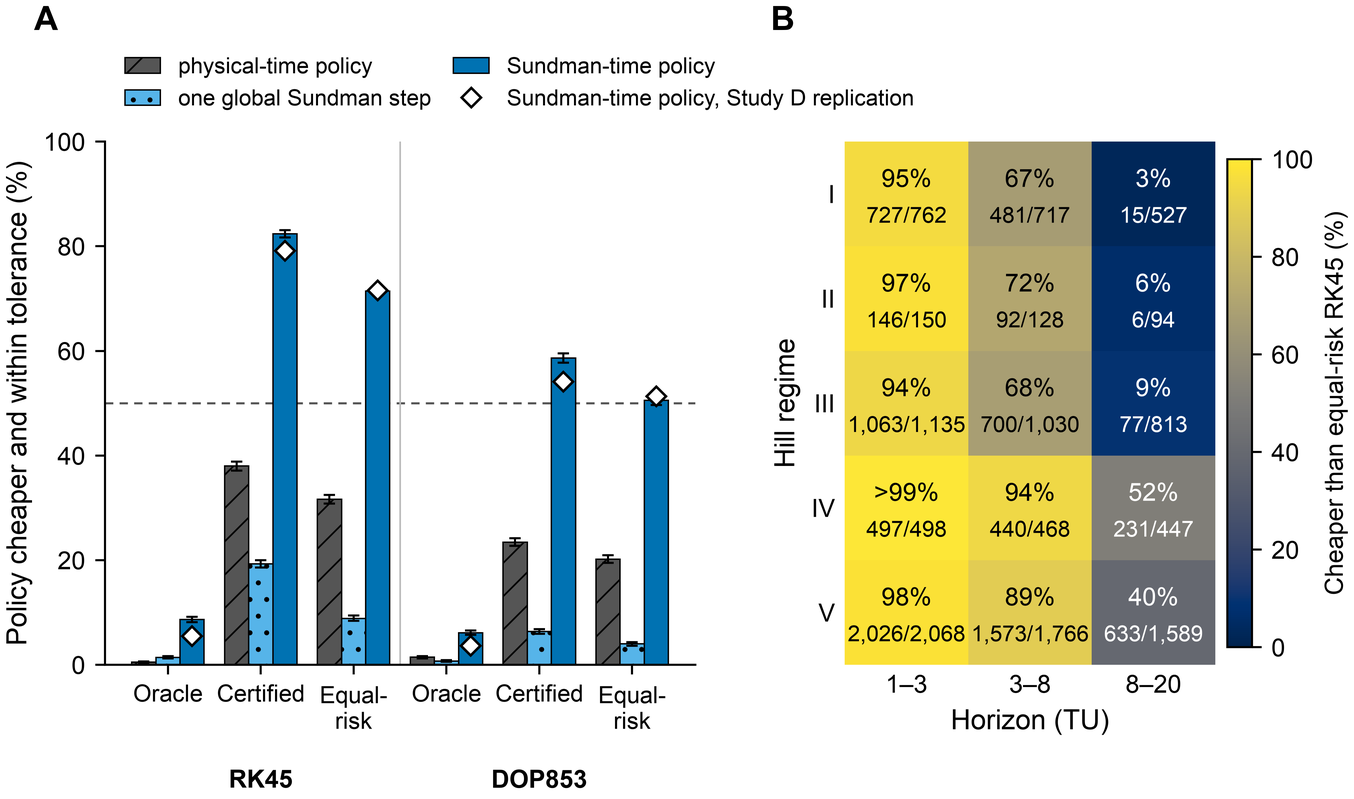
\includegraphics[width=\linewidth]{figures/draft/Fig5.png}\fi
\caption{{\bf The Sundman-time policy is cheaper than RK45 at equal risk except at long horizons in regimes I--III.}
(A) Share of trajectories on which each policy met the tolerance and cost less (overhead included) than RK45 and DOP853 at the oracle-tuned, certified and equal-risk tolerances: physical-time policy (grey, hatched), one global certified Sundman step (sky blue, dotted) and the Sundman-time policy (blue), Study C confirmation set ($n = 12,192$), with Clopper--Pearson 95\% intervals; open diamonds mark the Sundman-time policy on the Study D replication set ($n = 12,253$); dashed line, 50\%. (B) Share of trajectories on which the Sundman-time policy is cheaper than RK45 at the equal-risk tolerance, by Hill regime and horizon band, Study C confirmation set; each cell prints the share and its count $k/N$. TU, time unit.}
\label{fig5}
\end{figure}

The saving was not uniform (Fig~\ref{fig5}B). At horizons of 1--3 TU the policy was cheaper than equal-risk RK45 on more than 93\% of trajectories in every Hill regime (for example 727/762 in regime I and 2,026/2,068 in regime V), but at 8--20 TU it was cheaper on 15/527 (2.8\%) in regime I, 6/94 (6.4\%) in regime II and 77/813 (9.5\%) in regime III, where long chaotic horizons make the integration expensive and an adaptive controller well matched. The risk concentrated where it had in Study B: 299/2,222 trajectories (13.5\%) that passed within 0.05 DU of the Moon violated, against 13/3,462 (0.4\%) that stayed beyond 0.8 DU. Among the violations the median error was 1.7 times the tolerance and 35/535 (6.6\%) exceeded ten times the tolerance. Because the label and the certificate judge only the final position, we audited 1,000 re-run trajectories at 50 checkpoints: on 26/1,000 (2.6\%; 1.7--3.8\%) the maximum checkpoint error exceeded the tolerance while the final error did not.

A share counts trajectories, not evaluations, and the losses fell on the most expensive trajectories. In post hoc summaries of the sealed ledgers the policy used 1,434 evaluations per trajectory on average against 1,201 for equal-risk RK45 on the Study C confirmation set (1,643 against 1,318 on the Study D replication set), so the total cost of RK45 was 0.84 (95\% CI 0.81--0.86) and 0.80 (0.78--0.82) of the policy's (Table~\ref{table3}). Against the certified RK45 the totals were at parity in Study C (1.01, 0.98--1.04) and the policy lost in the replication (0.91, 0.88--0.93); against DOP853 it lost in total at both tolerances. The total-cost advantage was confined to short horizons: on the replication set equal-risk RK45 needed 1.48 (1.44--1.52) times the policy's evaluations at 1--3 TU, 0.97 (0.94--1.00) at 3--8 TU and 0.69 (0.67--0.71) at 8--20 TU, the band in which the policy spent 70\% of its evaluations; at 1--3 TU the policy also beat equal-risk DOP853 in total (1.26, 1.22--1.30). This is the horizon dependence that D2 found in compiled wall-clock time below; it is already present in evaluation counts. The share also depends on the sampling mixture (\nameref{S4_Table}). On the replication set it was 85--87\% for the $L_3$, $L_4$ and $L_5$ families, where the ratio of totals was at least 1.17, but 55--64\% for the $L_1$ and $L_2$ families and 55\% for near-Moon states (ratio of totals 0.70). Reweighting to a declared cislunar mixture (near-Moon, $L_1$ and $L_2$ states in equal parts) gave a share of 57.8\% (56.3--59.1\%) and a ratio of totals of 0.75 (0.73--0.77); equal weights for the seven sampling families gave 71.5\% and 0.81.

The 3,808 reference-divergent trajectories of the confirmation set (19.0\% of 20,000), excluded from the tests, were run separately. The Sundman-time policy ended in the same event type as the reference on 3,805/3,808 (99.9\%) and never passed through a body, because the transformation shrinks the step near the primaries.

\subsection*{Replication, and what carries the information}
Study D first asked whether the headline survives on data nobody had seen (D3). With the frozen Study C policy, its scale certified on 4,000 new calibration trajectories (0.800) and the comparators recalibrated on the same rows, the policy was cheaper than equal-risk RK45 on 8,768/12,253 trajectories of the replication set (71.6\%; 70.8--72.4\%, $p < 0.001$) at a violation rate of 330/12,253 (2.69\%; 2.41--3.00\%). Table~\ref{table3} shows that the shares against every comparator and in both locked evaluations agreed within a few points. One component of Study C did not replicate: the oracle Sundman step was cheaper than the oracle-tuned RK45 on 6,195/12,253 trajectories (50.6\%; 49.7--51.4\%, $p = 0.110$), so the threshold part of C3 was not met on the new data, while its mechanism (rank correlation 0.221 against 0.905) was.

\begin{table}[!ht]
\centering
\caption{{\bf The Sundman-time policy across four independent evaluations.}}
\small
\begin{tabular}{|L{1.55in}|L{0.95in}|L{0.95in}|L{0.8in}|L{0.8in}|}
\hline
 & \textbf{Study C confirmation} & \textbf{Study D replication} & \textbf{Study C lock} & \textbf{Study D lock} \\ \thickhline
Evaluation trajectories $N$ & 12,192 & 12,253 & 4,020 & 4,074 \\ \hline
Violations & 535 (4.4) & 330 (2.7) & 172 (4.3) & 100 (2.5) \\ \thickhline
Cheaper than RK45, equal-risk & 8,707 (71.4) & 8,768 (71.6) & 2,816 (70.0) & 2,863 (70.3) \\ \hline
Cheaper than RK45, certified & 10,045 (82.4) & 9,696 (79.1) & 3,264 (81.2) & 3,190 (78.3) \\ \hline
Cheaper than RK45, oracle-tuned & 1,058 (8.7) & 675 (5.5) & 360 (9.0) & -- \\ \hline
Cheaper than DOP853, equal-risk & 6,166 (50.6) & 6,284 (51.3) & 1,985 (49.4) & 1,991 (48.9) \\ \hline
Cheaper than DOP853, certified & 7,147 (58.6) & 6,628 (54.1) & 2,332 (58.0) & 2,200 (54.0) \\ \hline
Cheaper than DOP853, oracle-tuned & 747 (6.1) & 444 (3.6) & 247 (6.1) & -- \\ \thickhline
Median total cost, within tolerance & 235 & 255 & 251 & 260 \\ \hline
Median total cost, all (post hoc) & 251 & 267 & 267 & 272 \\ \thickhline
Ratio of totals, RK45 equal-risk (post hoc) & 0.84 (0.81--0.86) & 0.80 (0.78--0.82) & 0.85 (0.82--0.89) & 0.85 (0.82--0.88) \\ \hline
Ratio of totals, RK45 certified (post hoc) & 1.01 (0.98--1.04) & 0.91 (0.88--0.93) & 1.03 (0.99--1.07) & 0.97 (0.93--1.00) \\ \hline
Ratio of totals, DOP853 equal-risk (post hoc) & 0.69 (0.67--0.71) & 0.67 (0.65--0.69) & 0.70 (0.68--0.73) & 0.69 (0.67--0.72) \\ \hline
Ratio of totals, DOP853 certified (post hoc) & 0.78 (0.76--0.81) & 0.70 (0.68--0.72) & 0.80 (0.77--0.83) & 0.75 (0.72--0.78) \\ \thickhline
Certified scale & 0.872 & 0.800 & 0.872 & 0.800 \\ \hline
\end{tabular}
\begin{flushleft} Entries are counts $k$ of the $N$ evaluation trajectories with the percentage in parentheses. Violations: the policy run ended more than 100 km from the reference, collided, escaped or failed. Cheaper rows: trajectories on which the policy met the tolerance and cost fewer right-hand side (RHS) evaluations, overhead included, than the adaptive solver at that tolerance; the oracle-tuned comparators were not run on the Study D lock set (--). Median total cost: policy cost in RHS evaluations, overhead included, over the trajectories that met the tolerance (as preregistered) and over all trajectories (post hoc). Ratio of totals (post hoc summary of the sealed ledgers): comparator evaluations summed over all evaluation trajectories divided by the policy's total, overhead and violating runs included, with 95\% bootstrap intervals over trajectories; below 1, the policy used more evaluations in total. Overhead charged: 15.04 RHS-equivalents (Study C sets and Study D replication), 16.09 (Study D lock, re-measured in Study D). Charging 16.09 in every column lowers the equal-risk RK45 counts of the first three columns by 37, 28 and 11 (to 71.1, 71.3 and 69.8\%), charging 15.04 in the last raises it by 11 (70.5\%), and no ratio of totals moves by more than 0.001.
\end{flushleft}
\label{table3}
\end{table}

D1 asked whether a model is needed at all, since the Sundman transformation is a century old and the periapsis features are physics (Fig~\ref{fig6}A). Each arm was certified by the same rule on the same 4,000 calibration trajectories and charged its own overhead measured in one session. The 25-tree policy was cheaper than the best four-coefficient rule (horizon, Hill regime and periapsis radius) by 0.0715 dex (95\% CI 0.0695--0.0736), about 18\%, and cheaper on 8,040/11,565 paired trajectories (69.5\%; D1, $p < 0.001$). The rule using only the horizon was 0.163 dex behind, and one global fictitious step for all trajectories 0.274 dex behind on the replication set. Measured on the same confirmation set (post hoc, same protocol), the global step was 0.269 dex (0.266--0.273) behind, so the four-coefficient rule recovered 73\% (95\% CI 73--74\%) of the saving that the model achieves over a single global step. The tree structure was not what bought the rest: the linear model on the 33 engineered features came out 0.017 dex (0.016--0.019) cheaper than the trees on 11,569 paired trajectories, at a higher realized risk (579/12,239, 4.7\%, against 317/12,239, 2.6\%); since the scale grid has a resolution of 0.038 dex, we read this as a tie. Against the adaptive solvers the margin of the model mattered: the model was cheaper than equal-risk RK45 on 8,589/12,239 trajectories (70.2\%) and the best rule on 6,485/12,239 (53.0\%); against equal-risk DOP853 the shares were 6,038/12,239 (49.3\%) and 4,223/12,239 (34.5\%). In total evaluations (post hoc) equal-risk RK45 needed 0.82 (0.80--0.84) of the model's total and 0.58 (0.56--0.60) of the rule's.

An exploratory importance analysis (Fig~\ref{fig6}B) refitted larger models with each feature group removed. For the Sundman-time target, removing the periapsis group raised the test mean squared error by 0.0048 (95\% CI 0.0045--0.0050) and the horizon by 0.0086 (0.0082--0.0091), while the proximity group ($r_{1}$, $r_{2}$, $r_{1}/r_{2}$) and the Jacobi group contributed nothing detectable. For the physical-time target the periapsis group was nine times as important by refit (0.0443). Adding FTLE to the five deployable groups lowered the Sundman-time error by 0.0023 (0.0020--0.0025) of 0.007, real but small information that costs an integration. Because the groups are correlated, drop-group refits were preferred over permutation importance~\cite{strobl2008}.

\begin{figure}[!h]
\ifdraftfigs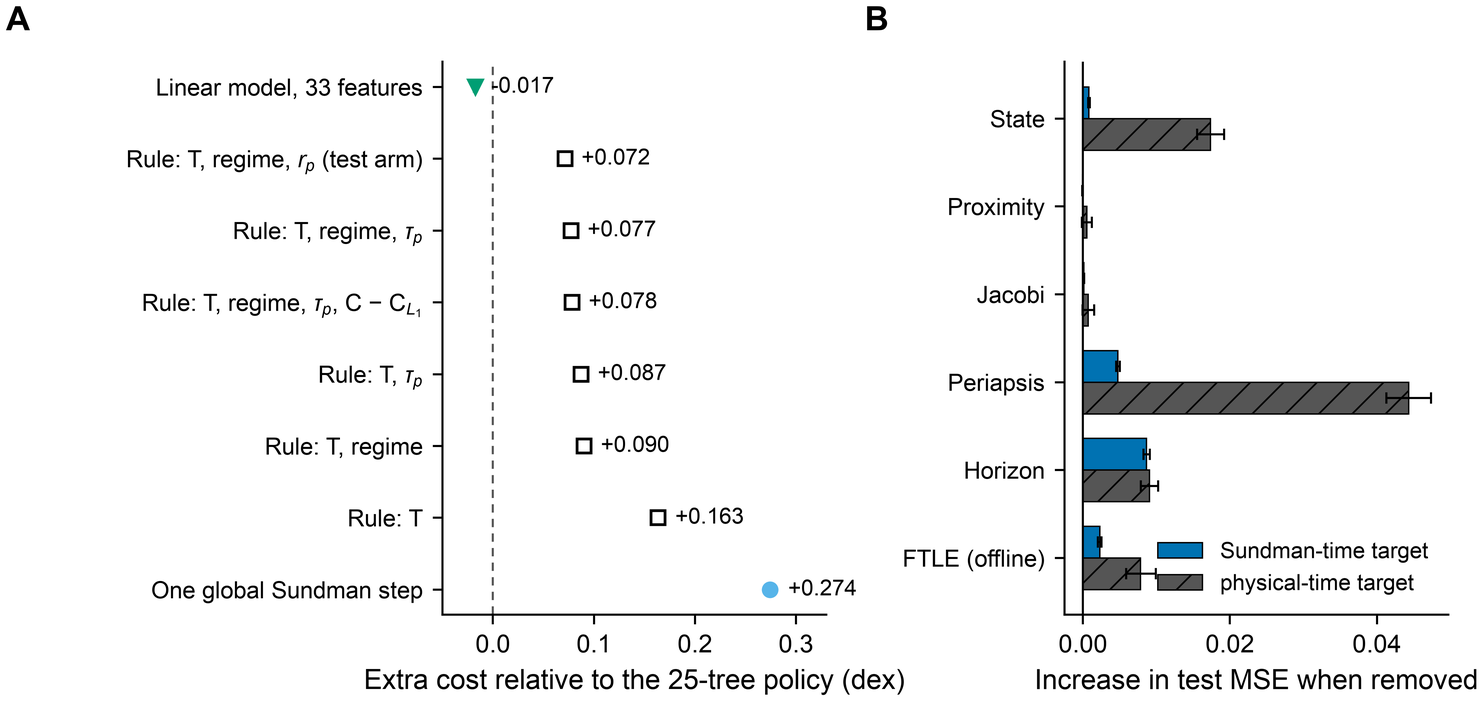
\includegraphics[width=\linewidth]{figures/draft/Fig6.png}\fi
\caption{{\bf Most of the saving comes from the time transformation and analytic periapsis information.}
(A) Mean extra cost in dex of each arm relative to the 25-tree Sundman-time policy, paired over trajectories that met the tolerance under both (Study D confirmation set, paired $n$ = 11,509--11,679), with 95\% paired bootstrap intervals; positive values mean the arm costs more. Rules are labelled by their inputs: horizon $T$, Hill regime, periapsis timescale $\tau_p$, periapsis radius $r_p$ and $C - C_{L_1}$; the test arm of D1 is marked. The linear model uses 33 engineered features. The single global certified fictitious step is from the Study D replication set ($n = 11,585$). (B) Exploratory: increase in test mean squared error (MSE) when a feature group is removed and the model refitted (200 trees of depth 6, 60,000 training rows, 16,239 test rows), for the Sundman-time target (blue) and the physical-time target (grey, hatched), with 95\% bootstrap intervals. FTLE was refitted together with all five deployable groups. FTLE, finite-time Lyapunov exponent.}
\label{fig6}
\end{figure}

\subsection*{Failure rates near the Moon and at long horizons}
The marginal certificate of Study C held on average and failed where the risk lands (D4, Fig~\ref{fig7}). With one scale for all trajectories, the evaluation trajectories of the replication set that passed within 0.05 DU of the Moon violated on 381/2,914 (13.1\%; 11.9--14.4\%), and the worst free stratum (regimes IV--V, far from the Moon, 8--20 TU) on 262/2,516 (10.4\%). Certifying a scale per stratum on the confirmation set put every one of the 17 strata at or below 3.1\% on the replication set (worst stratum 98/3,142, regimes IV--V far from the Moon at 1--3 TU; largest upper confidence bound 4.9\%), with an overall rate of 388/16,253 (2.4\%), while the policy remained cheaper than its equal-risk RK45 on 10,792/16,253 trajectories (66.4\%; 65.7--67.1\%; D4, $p < 0.001$). No stratum abstained. The improvement where trajectories actually passed close to the Moon was partial: 148/2,914 (5.1\%) violated below 0.05 DU and 91/2,013 (4.5\%) at 0.05--0.17 DU, because the osculating periapsis sees only part of the close passes.

\begin{figure}[!h]
\ifdraftfigs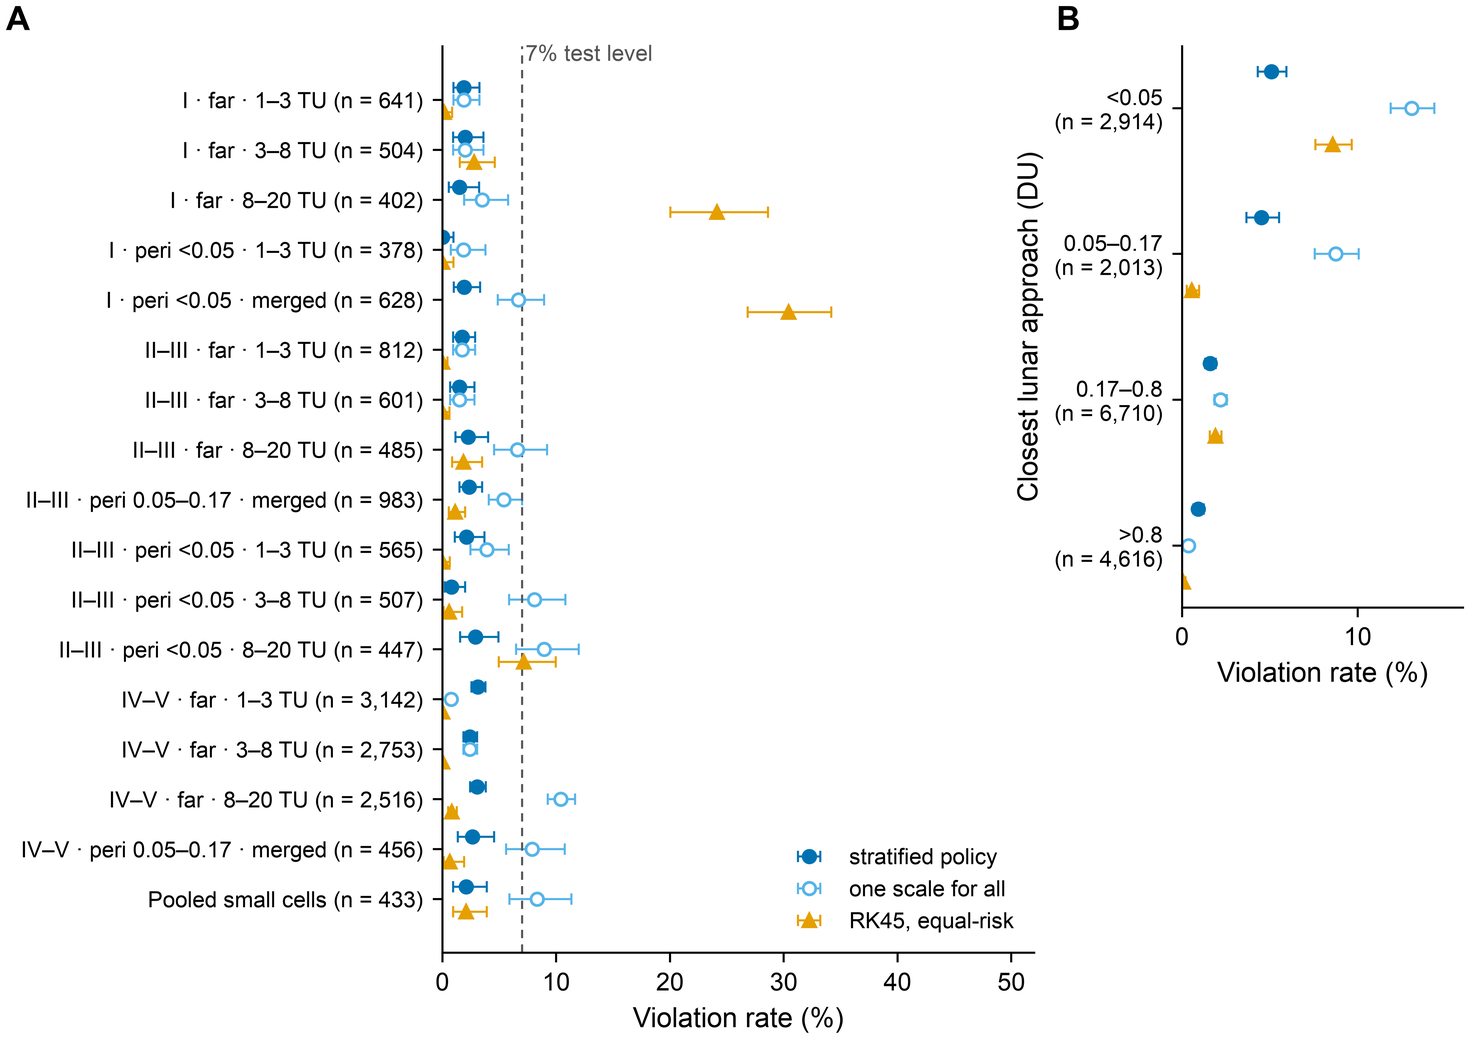
\includegraphics[width=\linewidth]{figures/draft/Fig7.png}\fi
\caption{{\bf A per-stratum certificate moves the risk out of the long-horizon and near-Moon tails.}
Study D replication set ($n = 16,253$), scales certified on the Study D confirmation set. (A) Violation rate in each of the 17 strata defined before integration (regime group $\cdot$ osculating lunar class $\cdot$ horizon band; evaluation $n$ in parentheses) for the stratified policy (filled blue circles), the policy with one scale for all (open sky-blue circles) and RK45 at the equal-risk tolerance of the stratified policy (orange triangles); bars are Clopper--Pearson 95\% intervals; dashed line, the 7\% test level. Lunar class: peri, osculating lunar periapsis below 0.05 DU or between 0.05 and 0.17 DU reached before the horizon; far, neither. Merged: horizon bands joined by the fixed merging rule. (B) The same rates by the closest lunar approach actually made, which is not known before integration. DU, distance unit; TU, time unit.}
\label{fig7}
\end{figure}

The equal-risk comparator was equal only on average. RK45 at the equal-risk tolerance violated on 97/402 (24.1\%) and 191/628 (30.4\%) trajectories of two regime-I strata (long horizons far from the Moon, and predicted close lunar passes), where the stratified policy violated on 6/402 (1.5\%) and 12/628 (1.9\%). In an exploratory post hoc comparison, RK45 certified per stratum by the same rule had an overall violation rate of 238/16,253 (1.5\%), and the stratified policy was cheaper than it on 9,137/16,253 trajectories (56.2\%; 55.5--57.0\%); against DOP853 certified per stratum it was cheaper on only 3,821/16,253 (23.5\%). In a second exploratory analysis of the 163 trajectories with the largest $\lambda T$, where both references agreed to 0.23 km, the policy violated on 41/163 (25.2\%; 18.7--32.5\%) against 317/12,239 (2.6\%) overall: its risk concentrates in the chaotic tail, and the error is the policy's, not the reference's.

\subsection*{Compiled wall-clock time}
D2 asked whether the evaluation-count result survives in compiled wall-clock time. It did not over the full horizon range (Fig~\ref{fig8}A). Against compiled Dormand--Prince 5(4) with a PI controller at the equal-risk tolerance, the throughput ratio over 12,239 trajectories was 0.885 (95\% CI 0.862--0.908; $p = 1.000$), although the policy was faster on 9,565/12,239 trajectories (78.2\%; median per-trajectory ratio 1.48). The total was dominated by long horizons. By horizon band the ratio was 1.61 at 1--3 TU (policy faster on 4,634/4,660), 1.02 at 3--8 TU (3,564/4,025) and 0.75 at 8--20 TU (1,367/3,554). Against compiled DOP853 at equal risk the ratio was 0.642 (0.625--0.658). The evaluation-count and wall-clock rankings agreed trajectory by trajectory (Spearman 0.99), and the cost per evaluation was at parity (22.4 ns for the policy, 23.1 ns for the comparator). The first implementation, which reused the Study C kernel, gave a ratio of 0.595 because the Sundman step evaluated extra square roots in every stage and its landing steps allocated memory (26.6 against 18.7 ns per evaluation); evaluation counts alone had hidden this cost. In batches of $10^{3}$ to $10^{5}$ trajectories on one or ten threads the ratio stayed between 0.82 and 0.91 (Fig~\ref{fig8}B), and modelled lock-step execution gave both methods similar lane efficiency (about 0.55, 0.31 and 0.18 at 2, 4 and 8 lanes with random batching).

\begin{figure}[!h]
\ifdraftfigs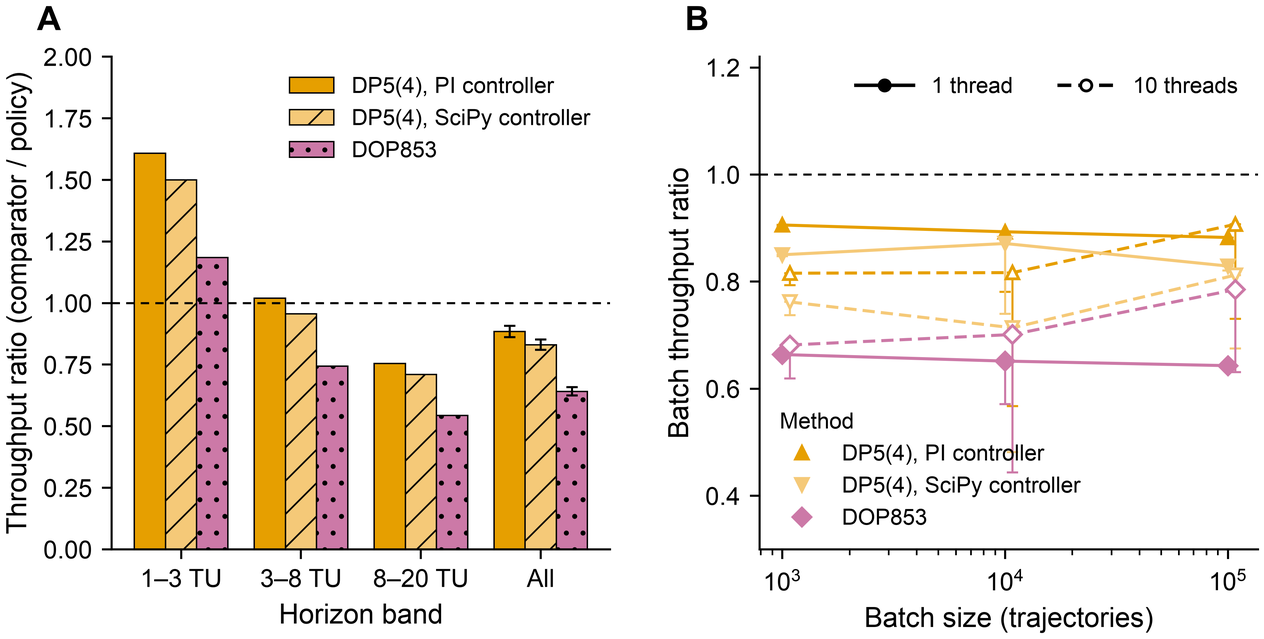
\includegraphics[width=\linewidth]{figures/draft/Fig8.png}\fi
\caption{{\bf The policy is faster in compiled wall-clock time only at short horizons.}
Apple M5, Study D confirmation set ($n = 12,239$). (A) Single-thread throughput ratio (total comparator time over total policy time; above 1 favours the policy; dashed line, parity) by horizon band and overall, against compiled Dormand--Prince 5(4) with a PI controller (the primary comparator), Dormand--Prince 5(4) with SciPy's controller and DOP853, each at its equal-risk tolerance; error bars on the overall ratios are 95\% bootstrap intervals over trajectories. (B) Batch throughput ratio against batch size on 1 thread (solid lines, filled markers) and 10 threads (dashed lines, open markers); markers are medians over 7 repeats and whiskers extend down to the worst repeat. PI, proportional--integral step controller; TU, time unit.}
\label{fig8}
\end{figure}

\subsection*{Periodic orbits and chaos}
D5 asked whether the frozen policy transfers to structured orbits it was not trained on. It did not (Fig~\ref{fig9}A). Over 1,647 in-range runs of 11 JPL families (942 members retained after the closure checks), the family-balanced violation rate was 70.0\% (95\% CI 67.8--72.3\%; 976/1,647 runs pooled; $p = 1.000$ against the 10\% level). The vertical and axial families violated on 98--102 of 102 runs each (96--100\%), the Lyapunov families on 80/102 ($L_1$) and 59/70 ($L_2$), and the halo, distant retrograde, butterfly and resonant families on 33--47\% of runs (counts per family in \nameref{S2_Table}). The failure was one of prediction (Fig~\ref{fig9}B): against the largest passing fictitious step of each run, the policy's raw step was too long by 0.15 dex in the median and by 0.3--0.5 dex on the vertical, axial and Lyapunov families, but within 0.07 dex on the halo, distant retrograde, butterfly and resonant families, whose violations came from unstable members. On a vertical $L_2$ member the Sundman-time RK4 converged at fourth order to the reference as the step shrank: the integrator was right and the step was wrong. A scale recalibrated on the disjoint dry-run sample (0.183 instead of 0.872) brought the violation rate to 3.5\% (\nameref{S2_Table}) at a median total cost of 3,299 evaluations, never cheaper than RK45. The comparators were not safe on these orbits either: RK45 at the Study C certified tolerance violated on 8--50\% of the runs of each family and at the equal-risk tolerance on 26--66\%, and the policy violated more often than equal-risk RK45 in every family.

\begin{figure}[!h]
\ifdraftfigs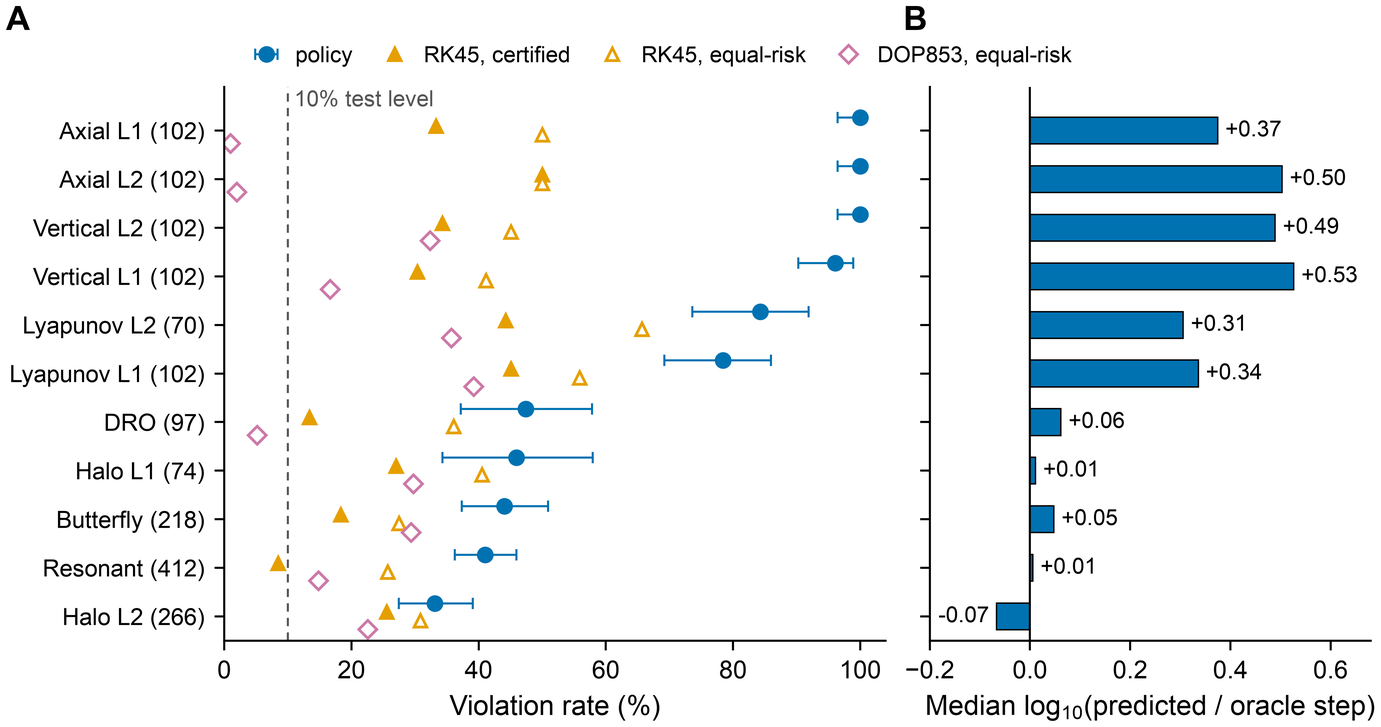
\includegraphics[width=\linewidth]{figures/draft/Fig9.png}\fi
\caption{{\bf On periodic-orbit families outside the training population the predicted step is too long.}
Frozen Study C policy and comparator tolerances applied to 1,647 runs (horizons of 1, 2, 5, 10 or 20 periods lying within 1--20 TU) of 11 Earth--Moon families from the JPL Three-Body Periodic Orbits API; number of runs per family in parentheses. (A) Violation rate per family for the policy (blue circles, Clopper--Pearson 95\% intervals), RK45 at the certified tolerance (filled orange triangles), RK45 at the equal-risk tolerance (open orange triangles) and DOP853 at the equal-risk tolerance (open diamonds); dashed line, the 10\% test level. (B) Median $\log_{10}$ ratio of the policy's raw fictitious step to the largest passing fictitious step of the same run; positive values mean the predicted step is too long. DRO, distant retrograde orbit; JPL, Jet Propulsion Laboratory; TU, time unit.}
\label{fig9}
\end{figure}

Finally, we asked where the failures sit relative to the chaotic structure of phase space (exploratory; Fig~\ref{fig10}). On three planar surfaces of section, which are themselves outside the sampled population (violations on 1,522/5,018, 1,563/5,457 and 1,600/6,211 grid points, 25.8--30.3\%), the FTLE of a grid point separated violations from non-violations with an AUC of 0.93, 0.92 and 0.93 at $C = 3.19$, 3.10 and 2.95. The four lowest FTLE deciles were almost free of violations and the top decile violated on 84--97\% of points. The violations lay in the near-Earth region and along the FTLE ridges, where trajectories are both fast and sensitive. FTLE explains the failures after the fact, but it requires the integration the policy is meant to avoid.

\begin{figure}[!h]
\ifdraftfigs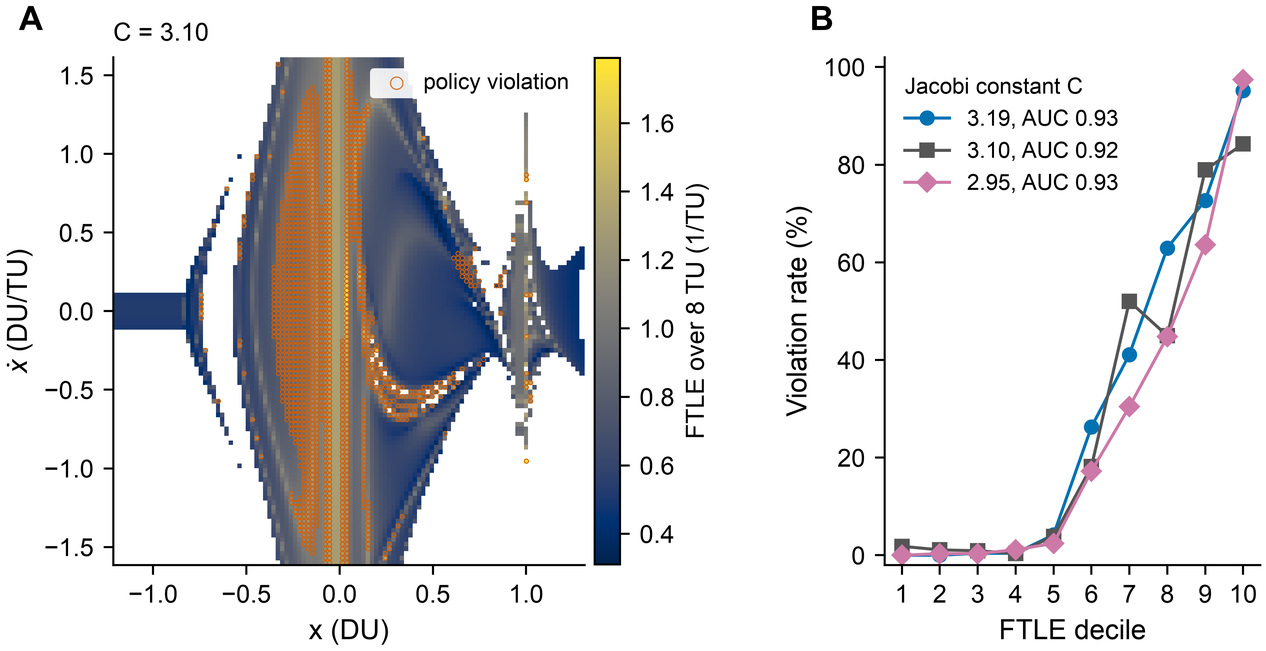
\includegraphics[width=\linewidth]{figures/draft/Fig10.png}\fi
\caption{{\bf Policy failures lie on high-FTLE ridges of the surface of section.}
Exploratory. Frozen Study C policy on the surface of section $y = 0$, $z = \dot{z} = 0$, $\dot{y} > 0$, on a $110 \times 110$ grid in $(x, \dot{x})$ with a horizon of 8 TU. (A) FTLE over 8 TU at $C = 3.10$ (colour) with policy violations as open vermillion circles (1,563 of 5,457 points); white, energetically inaccessible or reference not reaching the horizon. (B) Violation rate by FTLE decile at $C = 3.19$, 3.10 and 2.95 (5,018, 5,457 and 6,211 points), with the area under the receiver operating characteristic curve (AUC) of FTLE for the violations. DU, distance unit; FTLE, finite-time Lyapunov exponent; TU, time unit.}
\label{fig10}
\end{figure}

\section*{Discussion}
The hypothesis this project started from, that the FTLE, the distance to the primaries and the Jacobi constant govern how hard a trajectory is to integrate, held only after the fact. FTLE separates the failures of the final policy well (AUC 0.92--0.93), but it costs more than an adaptive solve, and removing it from the features changed neither prediction quality (Study A) nor much of the test error once the time transformation was in place (Study D). The second hypothesis, that a single physical step pays a penalty that grows with the range of timescales along the trajectory, was supported (Study B), and the intervention it suggested removed the dependence (Study C) and replicated (Study D). What made a pre-run step affordable was not a better learner but a change of time variable together with analytic information about the next close approach.

Our interpretation of the mechanism, which the studies support but did not test directly, is as follows. A fixed physical step must be short enough for the fastest part of the trajectory, so its cost scales with $T\max\tau^{-1}$, whereas an adaptive solver's cost scales with $\int\tau^{-1}\dd t$; their ratio is the timescale range $\Delta_{\tau}$, and the slope of nearly 1 between $\log_{10}\Delta_{\tau}$ and the paradigm gap is what this argument predicts. In Sundman time the step is proportional to the local timescale, so the remaining question is how fine the fictitious step must be, a quantity with a much narrower spread (0.33 dex against 0.91 dex for the physical step). The periapsis features supply the one piece of the future that matters most, whether and how closely the trajectory will pass a body before $T$. The residual failures are those this two-body picture cannot see: strong three-body perturbations on chaotic, long-horizon trajectories and close passes that the osculating orbit does not predict.

These results fit the literature on adaptive integration. Learned controllers that act during the run~\cite{dellnitz2023,sazulibarrena2025} see the trajectory and can correct their step; a pre-run choice cannot, and the information analysis of Study B shows that what it lacks is information about the future rather than precision about the present. Step criteria based on the local orbital timescale~\cite{pham2024} and time-transformed integrators~\cite{mikkola1999,preto1999,wang2020} encode the same physics that our rules and features recover, and a four-coefficient rule recovering three quarters of the saving is consistent with that. IAS15~\cite{rein2015} is not designed for a 100 km tolerance: in an exploratory comparison on 300 trajectories, at the loosest accuracy parameter that met the tolerance (the edge of the searched range), it took a median of 217 $\mu$s per trajectory against 6.4 $\mu$s for the compiled policy, about 29 times longer in total; part of that is per-call overhead from Python, so the factor bounds the algorithmic gap from above. Finally, the weak-baseline critique~\cite{mcgreivy2024} applies directly. Our headline comparison is against RK45 at a tolerance chosen to give the same marginal risk, which is a fair but not the strongest baseline: the policy did not beat DOP853 at equal risk (6,166/12,192, 50.6\%), nor either solver at an oracle tolerance, and over the full horizon range it was neither cheaper in total evaluations than equal-risk RK45 nor faster in wall-clock time. The preregistered share hid the first of these: it counts trajectories, while the cost of a batch is set by its longest trajectories.

The limitations, in order of likely impact, are these. (a) Distribution shift: the policy is unsafe on structured orbits outside its training population (D5), and its risk is concentrated in the high-$\lambda T$ tail even inside it. (b) Scope: one system, one tolerance (100 km) and one horizon range (1--20 TU); how the conclusions move with the tolerance is unknown. (c) The sampling mixture is synthetic, so every share is specific to it; a mission catalogue would weight Hill regimes and horizons differently, and a mixture of near-Moon and $L_1$/$L_2$ states alone lowered the share to 58\% (post hoc). (d) The label and the certificate judge only the final position; 26/1,000 audited runs (2.6\%) exceeded the tolerance in mid-run while ending within it. (e) About 19\% of each draw, trajectories whose reference collides or escapes, are outside the cost tests; the policy matched the event type on 3,805/3,808 of them, but its cost there was not compared. (f) Timing is from one machine and one compiler, in one session started with a relaxed load guard, with no GPU measurement. (g) The CR3BP itself differs from the real Earth--Moon ephemeris by 2,000--50,000 km at the horizons studied, so the tolerance describes integrator error inside the model only. (h) The oracle-tuned adaptive solvers and DOP853 at equal risk were not beaten. (i) Collisions were checked only at step endpoints; a long physical step can cross the Moon without registering. This cannot happen to the Sundman-time policy, whose steps shrink near the bodies, but it can hide collisions of the physical-time arms.

We state the practical implication as a hypothesis for future testing: pre-run step selection in Sundman time could reduce the cost of short-horizon dispersion studies (horizons of about 1--3 TU, where the policy was cheaper in total evaluations and in compiled wall-clock time; at 3--8 TU it was at parity) whose initial conditions come from a known, sampled population, provided that the scale is certified per stratum and that trajectories outside the population or with long horizons are handed to an adaptive solver. Nothing in our data supports using a pre-run step for structured orbit families without retraining or for long chaotic propagations.

\section*{Conclusions}
A single step chosen before the run by a learned model, in physical time, was never cheaper than adaptive integration in the spatial Earth--Moon CR3BP once its overhead and safety margin were counted: 0 of 14,161 trajectories. The decomposition of the cost gap showed that the penalty of any fixed physical step tracks the range of timescales along the trajectory. A Sundman time transformation removed that dependence, and a small model with analytic two-body periapsis features was then cheaper than RK45 at equal marginal risk on about 71\% of trajectories, in the confirmation set and in an independent replication, with its marginal failure rate certified below 5\% at confidence 0.9, and with a per-stratum certificate that kept every stratum at or below 3.1\% on new data. Cheaper on most trajectories is not cheaper in total: over horizons of 1--20 TU the policy used 19--25\% more evaluations than equal-risk RK45 (post hoc), and its total-cost advantage, with RK45 needing 1.48 times as many evaluations, was confined to horizons of 1--3 TU. Most of the per-trajectory saving comes from physics: a four-coefficient rule recovers about three quarters of the model's saving over one global step, and a linear model ties the trees. The result does not extend to DOP853, to oracle-tuned tolerances, to total evaluations or compiled wall-clock time over 1--20 TU, or to periodic-orbit families outside the training population.

Future work could test the tolerance and horizon dependence of these conclusions; train on, or abstain for, periodic-orbit families; replace the Sundman function by a regularizing Kustaanheimo--Stiefel transformation~\cite{kustaanheimo1965} near the Moon; move to an ephemeris model and to other mass ratios; certify a path error rather than an endpoint error; and measure batched execution on GPUs.

\section*{Acknowledgments}
Trajectory data for the fidelity check were obtained from the JPL Horizons system, and periodic-orbit initial conditions from the JPL Three-Body Periodic Orbits API, both provided by the Solar System Dynamics Group of the Jet Propulsion Laboratory.

\nolinenumbers

\bibliography{references}

\section*{Supporting information}

\paragraph*{S1 Appendix.}
\label{S1_Appendix}
{\bf Secondary methods and results.} Reference validation (Radau, DOP853 at the tightest tolerance, LSODA); label construction and the non-monotone labels; the Sundman landing rule and the $\tau_{c}$ sweep; the periapsis formulas including the near-circular and near-parabolic cases; the certification algorithm and the strata merging rule; the IAS15 baseline; the leapfrog symplecticity check; the ledger of reference-divergent trajectories; the endpoint audit; the exploratory lookahead and mass-ratio studies of Study B; the secondary hypotheses of Study A (H2, H4--H7) and the Sun--Earth transfer test; and the dated deviations of every preregistration.

\paragraph*{S1 Table.}
\label{S1_Table}
{\bf Conditional certificate by stratum.} For each of the 17 strata of D4: definition, certified scale, number of calibration and evaluation trajectories, violation counts and rates with Clopper--Pearson 95\% intervals for the stratified policy, the one-scale policy and RK45 and DOP853 at the equal-risk tolerance, and the share of trajectories on which the policy is cheaper.

\paragraph*{S2 Table.}
\label{S2_Table}
{\bf Periodic-orbit families.} D5 results by family, by stability index and by number of periods, and for the horizons beyond 20 TU (extrapolation).

\paragraph*{S3 Table.}
\label{S3_Table}
{\bf Full regression results.} Coefficients with bootstrap 95\% intervals and goodness of fit for the six physics rules and the linear model of D1, and the ordinary least-squares fit of the paradigm gap on the timescale range (T1).

\paragraph*{S4 Table.}
\label{S4_Table}
{\bf Post hoc cost summaries of the sealed ledgers.} For every policy ledger and adaptive comparator: the share cheaper, the ratio of totals and the mean $\log_{10}$ ratio with 95\% bootstrap intervals, by horizon band, Hill regime and sampling family; the declared alternative sampling mixtures; one overhead charged on every column of Table~\ref{table3}; the comparators certified by the policy's rule on a grid of matching cost resolution; equal-risk RK45 under other absolute-tolerance settings; and the spread over refits of the policy with other model seeds. None of these was a preregistered test.

\paragraph*{S1 Data.}
\label{S1_Data}
{\bf Data behind every figure and statistic.} One CSV file per figure and the per-trajectory ledgers from which every count, share, interval and test statistic in the article is computed.

\end{document}
